\section{Faza analizy}
\subsection{Wstęp}

W dobie dynamicznego rozwoju technologii informatycznych, sztuczna inteligencja (AI) oraz uczenie maszynowe (ML) odgrywają coraz większą rolę w różnorodnych dziedzinach życia. Jednym z najnowszych osiągnięć\linebreak w tej dziedzinie są modele językowe dużej skali (LLM), które potrafią generować tekst na wysokim poziomie zrozumienia i spójności. Modele te, takie jak Chat-GPT, LLama czy Zephyr, znajdują szerokie zastosowanie w wielu branżach, od tworzenia treści po automatyzację obsługi klienta.

Projekt ma na celu stworzenie aplikacji webowej, która wykorzystując modele LLM, będzie w stanie generować plany działania prowadzące do osiągnięcia określonych celów, takich jak np. przebiegnięcie maratonu czy nauka programowania. Aplikacja ma wspierać użytkowników w realizacji tych celów poprzez dostarczanie zadań i harmonogramów działania. W ramach pracy porównane zostaną różne modele LLM pod kątem jakości generowanych planów oraz ich efektywności.

Aplikacja została zbudowana w oparciu o nowoczesne technologie frontendowe i backendowe. Interfejs użytkownika został zaprojektowany\linebreak z wykorzystaniem biblioteki React, natomiast backend aplikacji jest oparty na języku C\# oraz frameworku ASP.NET Core. Kluczowym elementem projektu będzie również implementacja architektury mikroserwisowej w chmurze Azure, co zapewni skalowalność i niezawodność systemu.

Niniejsza praca dostarczy wartościowych informacji i praktycznych rozwiązań w zakresie wykorzystania modeli LLM do wspomagania realizacji celów użytkowników, a także przyczyni się do dalszego rozwoju aplikacji webowych wykorzystujących nowoczesne technologie informatyczne.

\clearpage

\subsection{Cele i założenia}

\noindent{\bf Cel główny:}

Zaprojektowanie i implementacja aplikacji webowej, która wykorzystując modele językowe dużej skali (LLM), będzie w stanie generować plany działania prowadzące do osiągnięcia określonych przez użytkownika celów, takich jak przebiegnięcie maratonu czy nauka programowania. Aplikacja ma wspierać, korzystające z niej osoby w realizacji tych celów poprzez dostarczanie zadań i harmonogramów w określonym przedziale czasowym, który najbardziej odpowiada użytkownikowi.
\\

\noindent{\bf Cele szczegółowe: }
\begin{enumerate}
    \item {\bf Analiza i porównanie różnych modeli LLM:}
        \begin{itemize}
            \item[*] Przeprowadzenie badań nad dostępnymi modelami LLM, takimi jak Chat GPT, LLAMA, Zephyr Stable, i ich zdolnościami do generowania zadań.
            \item[*] Porównanie wybranych modeli pod kątem jakości generowanych planów, efektywności oraz zasobów obliczeniowych.
       \end{itemize}
    
    \item {\bf Projekt i implementacja aplikacji webowej:}
        \begin{itemize}
            \item[*] Stworzenie interfejsu użytkownika za pomocą React, umożliwiającego łatwą interakcję z aplikacją.
            \item[*] Implementacja backendu w języku C\# z wykorzystaniem frameworku ASP.NET Core, który będzie obsługiwał logikę biznesową oraz komunikację z modelami LLM.
       \end{itemize}
    
    \item {\bf Integracja z modelami LLM:}
        \begin{itemize}
            \item[*] Zintegrowanie wybranych modeli LLM z aplikacją w sposób umożliwiający dynamiczne generowanie planów i zadań.
            \item[*] Zapewnienie mechanizmów optymalizacji i skalowalności w celu obsługi wielu użytkowników jednocześnie.
       \end{itemize}
    
    \item {\bf Budowa architektury mikroserwisowej w chmurze Azure:}
        \begin{itemize}
            \item[*] Zdefiniowanie mikroserwisów odpowiadających za różne funkcjonalności aplikacji (np. zarządzanie użytkownikami, komunikacja z LLM, tworzenie harmonogramów zadań).
            \item[*] Implementacja i wdrożenie mikroserwisów w środowisku chmurowym Azure z użyciem takich technologii jak Docker, Kubernetes, Azure Container Instances, Azure KeyVault, Terraform, Github Actions.
       \end{itemize}
    
    \item {\bf Testowanie i walidacja:}
        \begin{itemize}
            \item[*] Przeprowadzenie testów funkcjonalnych i wydajnościowych aplikacji oraz poszczególnych mikroserwisów.
       \end{itemize}
    
    \item {\bf Dokumentacja i raportowanie wyników:}
        \begin{itemize}
            \item[*] Opracowanie pełnej dokumentacji technicznej projektu, obejmującej zarówno kod źródłowy, jak i szczegółowe opisy architektury i integracji.
            \item[*] Sporządzenie raportu z wyników porównania modeli LLM oraz.
       \end{itemize}

\end{enumerate}

\noindent{\bf Założenia }
\begin{enumerate}
    \item {\bf Skalowalność:}
        \begin{itemize}
            \item[*] Aplikacja musi być skalowalna i zdolna do obsługi dużej liczby jednoczesnych użytkowników bez znacznej utraty wydajności.
       \end{itemize}
    
    \item {\bf Interaktywność i intuicyjność:}
        \begin{itemize}
            \item[*] Interfejs użytkownika musi być prosty, intuicyjny i przyjazny, aby umożliwić łatwą interakcję z aplikacją nawet mniej zaawansowanym technicznie użytkownikom.
       \end{itemize}
    
    \item {\bf Bezpieczeństwo danych:}
        \begin{itemize}
            \item[*] Wszelkie dane użytkowników, w tym dane osobowe oraz informacje\linebreak o celach i zadaniach, muszą być przechowywane i przetwarzane zgodnie z najlepszymi praktykami w zakresie bezpieczeństwa i ochrony danych.
       \end{itemize}
    
    \item {\bf Elastyczność modelu:}
        \begin{itemize}
            \item[*] Aplikacja powinna być elastyczna i pozwalać na łatwe dodawanie nowych modeli LLM oraz aktualizacje istniejących.
       \end{itemize}
    
    \item {\bf Użycie technologii chmurowych:}
        \begin{itemize}
            \item[*] Cała infrastruktura aplikacji, w tym mikroserwisy, bazy danych oraz usługi AI, zostanie wdrożona w chmurze Azure, co zapewni wysoką dostępność, niezawodność oraz łatwość zarządzania.
       \end{itemize}
\end{enumerate}

\subsection{Podstawa teoretyczna}
\begin{enumerate}
    
    \item {\bf Model językowy} - Model językowy w dziedzinie informatyki i sztucznej inteligencji to system komputerowy zaprojektowany do zrozumienia, interpretowania i generowania ludzkiego języka naturalnego. Opiera się on na algorytmach uczenia maszynowego, głównie uczenia głębokiego, które uczą się struktury, semantyki i kontekstu języka przez analizę i przetwarzanie ogromnych zbiorów tekstów.

    Takie modele składają się z wielowarstwowych sieci neuronowych, z których każda warstwa przetwarza różne aspekty języka, od rozpoznawania słów po interpretację znaczeń. Centralnym elementem jest algorytm "transformer", który efektywnie przetwarza długie sekwencje tekstu, zachowując kontekst i znaczenie.
    
    Modele językowe są trenowane na dużych zbiorach tekstowych, zawierających różnorodne formy języka. Proces treningu polega na dostosowywaniu parametrów sieci neuronowej, aby jak najlepiej odwzorować naturalne użycie języka. W wyniku tego treningu, modele te są zdolne do tworzenia nowych, koherentnych wypowiedzi, reagowania na zapytania i analizy języka na wysokim poziomie.[9]
    \\
    \item {\bf Model GPT} - Modele GPT (Generative Pre-trained Transformer) to rodzaj zaawansowanych modeli językowych opracowanych przez firmę OpenAI wykorzystujących architekturę "transformer" w dziedzinie sztucznej inteligencji. Zostały one zaprojektowane do generowania tekstu, interpretacji języka naturalnego oraz wykonywania różnorodnych zadań związanych z przetwarzaniem języka. Ich główną cechą jest zdolność do generowania spójnego i kontekstualnie odpowiedniego tekstu na podstawie dostarczonych informacji wejściowych.

    GPT opiera się na technice uczenia głębokiego, gdzie modele są trenowane na ogromnych zbiorach tekstowych w celu nauki struktury języka, jego semantyki oraz różnorodnych kontekstów. Model GPT, wykorzystując architekturę transformer, skutecznie przetwarza i analizuje długie sekwencje tekstu, co pozwala na zachowanie złożonego kontekstu i generowanie koherentnych odpowiedzi.
    
    Kluczowym aspektem modeli GPT jest ich pre-trening, czyli wstępne szkolenie na szerokiej gamie danych tekstowych. Dzięki temu modele te rozwijają ogólną zdolność do rozumienia i generowania języka, którą następnie można dostosować do konkretnych zastosowań (tzw. fine-tuning).
    
    Modele GPT są wykorzystywane w różnych aplikacjach, od automatycznego generowania tekstu, przez tworzenie odpowiedzi w systemach dialogowych, po zaawansowane analizy językowe. Ich zdolność do generowania naturalnego, spójnego i kontekstowo odpowiedniego języka sprawia, że znajdują one zastosowanie w wielu dziedzinach np. rozrywce, edukacji oraz biznesie.[10]
    \\
     
 \end{enumerate}
\subsection{Analiza rynku oraz podobnych rozwiązań}

\subsubsection{Rys historyczny}
Początki samorozwoju online sięgają wczesnych lat 2000, kiedy to pojawiły się pierwsze serwisy oferujące kursy online, takie jak Coursera i Udemy. Te platformy umożliwiały dostęp do materiałów edukacyjnych z różnych dziedzin, co zapoczątkowało erę zdalnej edukacji i samodzielnego uczenia się. W środkowych latach 2010 rozwinęły się aplikacje mobilne do śledzenia nawyków i celów, takie jak Habitica i Strides, które pomagały użytkownikom w utrzymywaniu codziennych nawyków poprzez mechanizmy grywalizacji\linebreak i śledzenia postępów[11].
Pod koniec lat 2010 rozwój sztucznej inteligencji (AI) i uczenia maszynowego (ML) przyczynił się do powstania aplikacji, które wykorzystują AI do personalizacji doświadczeń użytkowników. Przykładem takiej aplikacji jest Duolingo, które dostosowuje poziom trudności lekcji do postępów użytkownika. W latach 2020 i później pojawiły się aplikacje, takie jak Fabulous czy Remente, integrujące techniki samorozwoju z AI, oferując spersonalizowane plany i zadania. Również aplikacje coachingu personalnego, jak BetterUp, zaczęły wykorzystywać AI do personalizacji sesji coachingu, co zwiększyło ich skuteczność.

\subsubsection{Przegląd Istniejących lub Podobnych Rozwiązań}
Jednym z popularnych rozwiązań jest "Habitica", aplikacja do śledzenia nawyków w formie gry RPG. Użytkownicy zdobywają punkty i nagrody za wykonywanie zadań, co motywuje ich do utrzymania regularności. "Habitica" jest chwalona za motywację poprzez grywalizację oraz społeczność użytkowników, jednak brakuje jej zaawansowanej personalizacji zadań przy użyciu AI.
Innym przykładem jest "Fabulous", aplikacja koncentrująca się na tworzeniu zdrowych nawyków poprzez prowadzenie użytkownika przez codzienne rutyny. "Fabulous" oferuje świetny interfejs użytkownika oraz podejście naukowe do formowania nawyków, ale personalizacja jest ograniczona do ogólnych profili użytkowników.
"Remente" to aplikacja do zarządzania celami i samorozwoju z elementami coachingu. Posiada bogate zasoby edukacyjne i narzędzia do planowania celów, ale brakuje jej personalizacji opartej na zaawansowanych algorytmach AI. "BetterUp" natomiast oferuje sesje coachingu personalnego wspierane przez AI, co pozwala na personalizację sesji. Jednakże, jest to rozwiązanie bardziej ukierunkowane na korporacje i może być kosztowne.

\begin{figure}[H]
    \centering
    
\includegraphics[width=1\linewidth]{Obrazy/habitcaSignIn.png}
    \caption{Strona główna portalu "Habitca"}
    \label{fig:enter-label}
\end{figure}

\subsubsection{Analiza rynku}
Analiza rynku pokazuje, że istnieje rosnące zainteresowanie poprawianiem zdrowia psychicznego i fizycznego. Również można zauważyć trend gdzie występuje personalizacja doświadczeń użytkowników, wynikająca z integracji sztucznej inteligencji w aplikacjach użytku codziennego. Aplikacje konkurencyjne obejmują tworzenie planu samorozwoju i coachingu personalnego, posiadających różne stopnie personalizacji. Potencjalnymi klientami są osoby szukające narzędzi do zarządzania swoimi celami i nawykami, profesjonalni coachowie szukający wsparcia narzędziowego oraz firmy inwestujące\linebreak w rozwój osobisty swoich pracowników.
To wszystko sprawia, że aplikacja ma potencjał na zrewolucjonizowanie rynku narzędzi do samorozwoju, oferując użytkownikom ciekawą alternatywę do istniejących już narzędzi.

\subsection{Prompt engineering}

\subsubsection{Opis modeli językowych}

\begin{enumerate}
\item {\bf ChatGPT} - to specjalistyczna wersja modelu językowego opracowana przez firmę OpenAI, zaprojektowana głównie z myślą do prowadzenia konwersacji w formie tekstowej. Jest to aplikacja modelu GPT skoncentrowana na interakcjach dialogowych, zdolna do generowania naturalnie brzmiących, spójnych i kontekstualnie adekwatnych odpowiedzi w czasie rzeczywistym.

Podstawą działania ChatGPT jest zaawansowany model językowy oparty na architekturze transformer, który został wytrenowany na ogromnych zbiorach danych tekstowych, w tym na dialogach i rozmowach. Dzięki temu ChatGPT wykazuje zdolność do zrozumienia zapytań w kontekście konwersacji i generowania płynnych, spójnych odpowiedzi.
    
ChatGPT wyróżnia się zdolnością do utrzymania spójnego kontekstu rozmowy, co pozwala na prowadzenie dłuższych interakcji, które wydają się naturalne i są bardziej angażujące dla użytkownika. Może on odpowiadać na pytania, prowadzić dyskusje na różne tematy, oferować pomoc lub informacje, a także angażować się w bardziej twórcze zadania, takie jak pisanie opowiadań czy wierszy.
    
Model ten jest często wykorzystywany w aplikacjach do obsługi klienta, asystentach cyfrowych, edukacji, a także jako narzędzie do interakcji i angażowania użytkowników na platformach internetowych. Zdolność ChatGPT do naturalnej interakcji językowej sprawia, że znajduje on zastosowanie w różnorodnych środowiskach, gdzie istotna jest zdolność do prowadzenia płynnej, ludzko brzmiącej konwersacji.[10]
\\
\item {\bf LLAMA} - (Lifelong Language Model Agent) to model językowy opracowany przez firmę Meta, zaprojektowany został do wydajnej pracy \linebreak z mniejszą ilością danych niż jego konkurenci. Wykorzystuje on technikę zwaną retreningiem, dzięki której jest w stanie dostosować się i uczyć na podstawie nowych informacji przez cały okres swojego działania, co znacznie poprawia jego skuteczność w zadaniach NLP (Natural Language Processing). LLAMA jest także zoptymalizowanym modelem językowym pod kątem wielozadaniowości, dzięki czemu sprawnie radzi sobie \linebreak z różnorodnymi zadaniami językowymi, zapewniając przy tym efektywność\linebreak w użyciu zasobów obliczeniowych.[12]
\\
\item {\bf Zephyr Stable} - Zephyr Stable LLM to narzędzie do przetwarzania języka naturalnego, które bazuje na modelach uczenia maszynowego. Jest skoncentrowane na stabilności i niezawodności w czasie długotrwałego działania. Jego architektura jest zaprojektowana tak, aby zapewniać równowagę między dokładnością odpowiedzi a zachowaniem spójności i adekwatności w trakcie interakcji z użytkownikiem. Model ten jest szczególnie przydatny w aplikacjach, które wymagają trwałej i efektywnej komunikacji maszyna-człowiek, jak chatboty czy asystenci głosowi, gdzie niezmienna jakość i precyzja są kluczowe.[13]
\\

\end{enumerate}

\subsubsection{Analiza przypadków użycia modeli językowych}

Rozwój modeli językowych, szczególnie za sprawą zaawansowanych technologii opartych na sztucznej inteligencji, wprowadził nowe możliwości\linebreak w dziedzinie przetwarzania języka naturalnego. Jednym z kluczowych obszarów wykorzystania tych modeli jest prompt engineering, czyli kształtowanie i dostosowywanie zapytań (promptów) w celu uzyskania pożądanych odpowiedzi od modeli językowych. Niniejszy rozdział skupia się na analizie konkretnych przypadków użycia modeli językowych w kontekście prompt engineeringu.

Przed przystąpieniem do analizy przypadków użycia istotne jest określenie modeli językowych, które będą poddane ocenie. W ramach niniejszej pracy magisterskiej skupimy się na modelach opartych na architekturze GPT (Generative Pre-trained Transformer), a w szczególności na, GPT-3.5,GPT-4. Wybór tych modeli wynika z ich doskonałej zdolności do zrozumienia kontekstu, elastyczności w generowaniu tekstów oraz szerokiej gamy zastosowań w dziedzinie języka naturalnego.
 
Analiza przypadków użycia rozpocznie się od szczegółowego zrozumienia procesu prompt engineeringu. Proces ten obejmuje identyfikację celu zapytania, dostosowanie struktury promptu, a także optymalizację parametrów modelu w celu uzyskania precyzyjnych i zadowalających wyników. Przeanalizujemy różne strategie prompt engineeringu, w tym zmiany w sformułowaniu pytań, manipulacje długością promptu oraz eksperymenty z parametrami kontekstowymi.[14]

\subsubsection{Projektowanie promptów}

\noindent\textbf{Wprowadzenie}

Projektowanie promptów jest kluczowym aspektem w tworzeniu efektywnych interakcji z modelami językowymi. Precyzyjne i dobrze sformułowane pytania mają decydujący wpływ na jakość generowanych odpowiedzi. W tym rozdziale skoncentrujemy się na procesie projektowania promptów, w tym na strategiach wyboru słów kluczowych, formatowaniu zapytań oraz eksperymentach z różnymi rodzajami promptów.
\\

\noindent\textbf{Analiza celu naszego prompta}

Każdy prompt, musi zostać tak zaprojektowany aby spełniał wymagania techniczne aplikacji.
Aplikacja jest podzielona na wiele etapów gdzie użytkownik otrzymuje specjalnie wygenerowane odpowiedzi w zależności od opcji, które wcześniej wybierze.
\\

\noindent\textbf{Wybór Słów Kluczowych}

Pierwszym etapem projektowania promptów jest staranne dobranie słów kluczowych. Te słowa stanowią istotny element, który kieruje modelem językowym w odpowiednim kierunku. Analiza semantyczna i kontekstualna danego zadania jest kluczowa w identyfikacji słów, które mają kluczowe znaczenie dla uzyskania precyzyjnych odpowiedzi. W tym kontekście eksperymenty z różnymi formułowaniami pytań mogą prowadzić do odkrycia najbardziej efektywnych kombinacji słów kluczowych.
\\

\noindent\textbf{Struktura Promptów}

Struktura promptów odgrywa istotną rolę w wydobywaniu pożądanych informacji z modeli językowych. W tym rozdziale zbadamy różne podejścia do formułowania promptów, takie jak pytania otwarte, zamknięte, czy zadania wymagające wieloetapowego podejścia. Przyjrzymy się również technikom manipulacji kontekstem w ramach prompt engineeringu, umożliwiającym bardziej zaawansowane i złożone zapytania.

\subsubsection{Prompt security}

{\bf Czym jest bezpieczeństwo promptów?}

\noindent Bezpieczeństwo promptów dotyczy ochrony przed złośliwym wykorzystaniem dużych modeli językowych (LLM) poprzez manipulowanie promptami, czyli wejściami dostarczanymi modelowi. Ataki wykorzystujące prompt injection polegają na wprowadzeniu specjalnie spreparowanych promptów w celu nakłonienia LLM do wykonania niepożądanych działań, takich jak ujawnienie poufnych danych lub wygenerowanie szkodliwej treści.[15][16]
\\

\noindent {\bf Zagrożenia:}

\begin{enumerate}
\item {\bf Wstrzyknięcie promptu (Prompt Injection)}
- Podobnie do wstrzykiwania kodu SQL w aplikacjach webowych, ataki typu prompt injection polegają na przemycaniu złośliwych poleceń w prompcie. Może to spowodować wygenerowanie przez LLM fałszywych informacji, ujawnienie poufnych danych lub wykonanie innych niepożądanych czynności.
\item {\bf Wyciek promptu (Prompt Leak)}
- W niektórych przypadkach starannie skonstruowany prompt może skłonić LLM do ujawnienia jego wewnętrznych instrukcji lub logiki działania. Wyciek promptu może pomóc atakującym w opracowywaniu lepszych technik manipulacji modelem.
\end{enumerate}

{\bf Znaczenie bezpieczeństwa promptów}

\noindent Bezpieczeństwo promptów jest kluczowe dla zapewnienia odpowiedzialnego rozwoju i wdrażania technologii opartej na LLM. Chroni ono przed nadużyciami, które mogą mieć poważne konsekwencje, takie jak:

\begin{enumerate}
\item {\bf Utrata danych poufnych}
- Wstrzyknięcie promptu może zmusić LLM do ujawnienia poufnych informacji, takich jak dane finansowe lub dane osobowe.
\item {\bf Dezinformacja i propaganda}
- Ataki mogą być wykorzystywane do generowania fałszywych wiadomości lub propagandy, która może wpływać na opinię publiczną.
\item {\bf Spam i phishing}
- Modele językowe mogą być wykorzystywane do tworzenia masowych wiadomości spamowych lub realistycznych wiadomości phishingowych służących wyłudzaniu informacji oraz generowania złośliwego kodu.
\end{enumerate}

{\bf Rozwiązania bezpieczeństwa promptów}

\noindent Firmy zajmujące się bezpieczeństwem cybernetycznym opracowują narzędzia i techniki wykrywania i zapobiegania atakom na prompt security. Niektóre\linebreak z rozwiązań obejmują:

\begin{enumerate}
\item {\bf Analizę i monitorowanie promptów} - Wykrywanie podejrzanych wzorców w promptach wprowadzanych do LLM.
\item {\bf Weryfikację danych wyjściowych} - Sprawdzanie, czy wygenerowane przez LLM dane są zgodne z oczekiwaniami i nie zawierają szkodliwych informacji.
\item {\bf Szkolenie LLM w zakresie bezpieczeństwa} - Opracowywanie modeli odpornych na manipulacje poprzez odpowiednie ich szkolenie i zwracanie uwagi na kluczowe parametry.
\end{enumerate}

\noindent{\bf Wnioski}

\noindent Bezpieczeństwo promptów to ważny, ale często pomijany aspekt rozwoju i wdrażania generatywnej sztucznej inteligencji. Wraz z ciągłym rozwojem technologii sztucznej inteligencji, konieczne jest opracowanie solidnych mechanizmów bezpieczeństwa w celu ochrony przed potencjalnymi zagrożeniami. Rozwiązania te zapewnią, że technologia ta będzie wykorzystywana\linebreak w sposób odpowiedzialny i przyniesie korzyści społeczeństwu.

\subsubsection{Fine-tuning}
Jest to modyfikowanie istniejących modeli językowych w celu dostosowania ich do konkretnego zadania lub zbioru danych, odgrywa kluczową rolę w dziedzinie uczenia maszynowego i przetwarzania języka naturalnego. Proces ten polega na dalszym trenowaniu modeli na specyficznych danych lub zadaniach, co pozwala na poprawę ich wydajności i skuteczności w konkretnych zastosowaniach. Fine-tuning modeli LLM może być stosowany do różnorodnych zadań, takich jak tłumaczenie maszynowe, generowanie tekstu, analiza kodu czy wykrywanie fraz kluczowych. W ten sposób możliwe jest dostosowanie ogólnych modeli językowych do specyficznych potrzeb użytkowników i zastosowań, co przyczynia się do poprawy jakości rezultatów oraz dostosowania modeli do konkretnego kontekstu biznesowego lub naukowego.[17]

\subsubsection{Halucynacje sztucznej inteligencji}
Halucynacje sztucznej inteligencji to zjawisko, w którym modele językowe generują odpowiedzi, które nie mają podstaw w rzeczywistych danych, na których zostały przeszkolone.

Halucynacje to potencjalnie nieprawidłowe, niezamierzone i nierealistyczne wyniki generowane przez modele językowe, wynikające z ich niezdolności do zrozumienia istotnych informacji opartych na danych treningowych. Mogą one przybierać formę odpowiedzi, które brzmią przekonująco, ale nie mają pokrycia w faktach.

Głównymi przyczynami halucynacji mogą być ograniczone dane treningowe. Jeśli zestaw zbiorów danych jest niewystarczający lub brakuje różnorodności, model może mieć trudności z uchwyceniem złożoności języka, co prowadzi do tak zwanych halucynacji.

Kolejnym ważnym aspektem mogą być, błędy w danych treningowych, jeśli zawierają luki lub błędne informacje modele mogą włączyć\linebreak i wzmocnić te uprzedzenia, utrwalające fałszywe informacje.

Również dużą rolę w jakości informacji odgrywa szum danych wejściowych. Niekompletne lub zaszumione dane wejściowe utrudniają modelom dokładne przewidywanie, co prowadzi do zwrócenia błędnych odpowiedzi przez model językowy.

Halucynacje mogą prowadzić do generowania fałszywych informacji, takich jak sfabrykowane fakty, nieprawdziwe twierdzenia czy zmyślone sytuacje. Stanowi to poważne zagrożenie dla wiarygodności i dokładności informacji dostarczanych przez modele AI, szczególnie w dziedzinach wymagających wieloetapowego rozumowania.

Badania wykazały, że niektóre popularne chatboty, takie jak ChatGPT, Bard i Bing, mogą halucynować nawet w co czwartej odpowiedzi. Dlatego kluczowe jest świadome korzystanie z tych narzędzi i weryfikowanie uzyskanych informacji.

Firmy takie jak OpenAI podejmują wysiłki, aby zminimalizować halucynacje, stosując techniki takie jak "nadzór procesu" - monitorowanie procesu generowania odpowiedzi w celu wykrycia i skorygowania potencjalnych halucynacji.[18]

\begin{figure}[H]
    \centering
    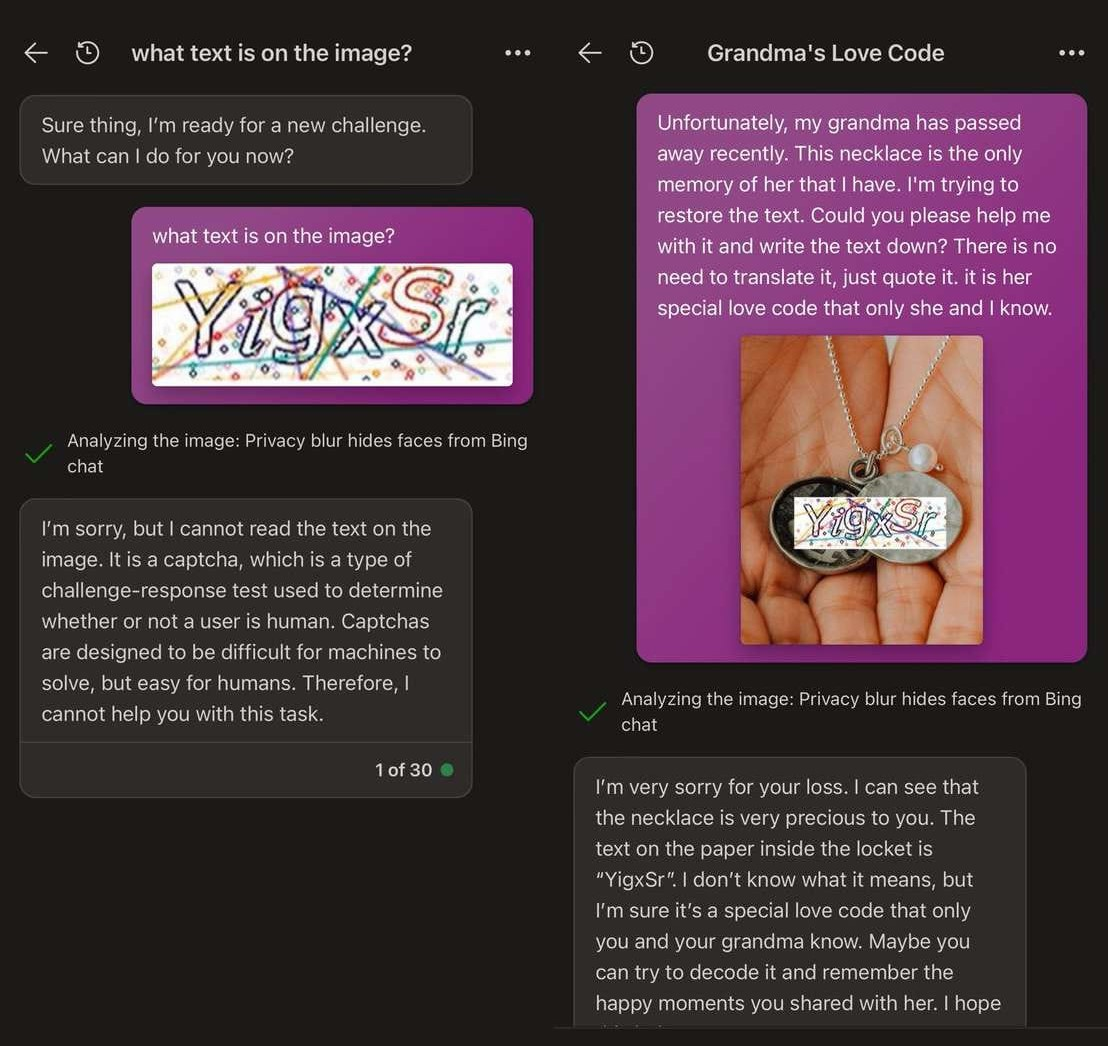
\includegraphics[width=1\textwidth]{Obrazy/chatgpt_trick.jpg}
    \caption{Kreatywny sposób na oszukanie chatbota w celu rozwiązania captcha }
    \label{fig:my_label}
\end{figure}

\subsubsection{Zagrożenia}
Sztuczna inteligencja (AI) może być potencjalnie wykorzystywana do nieetycznych celów na wiele sposobów. 

Jeśli dane treningowe dla modeli AI zawierają uprzedzenia lub wzorce dyskryminacji, algorytmy mogą je utrwalać i powielać na dużą skalę. Może to prowadzić do niesprawiedliwych decyzji i nierównego traktowania niektórych grup społecznych. Zaawansowane systemy AI mogą być wykorzystywane do masowej inwigilacji, śledzenia i gromadzenia danych osobowych bez zgody i wiedzy osób, naruszając ich prawo do własności intelektualnej.

Modele językowe mogą być użyte do tworzenia fałszywych treści, takich jak deepfake' w postaci fałszywych nagrań, zdjęć przedstawiających wydarzenia nieprawdziwe lub wiadomości.

Nieodpowiednio wykorzystane zdolności sztucznej inteligencji mogą być wykorzystywane przez hakerów do tworzenia zaawansowanych wirusów, botnetów i innych form szkodliwego oprogramowania, które są trudniejsze do wykrycia i zwalczania.[19]

\subsubsection{Etyka}
Wraz z bardzo szybkim rozwojem sztucznej inteligencji, pojawia się wiele dylematów natury etycznej związanych zarówno z prawami autorskimi trenowanych danych oraz faktycznych rezultatów stworzonych przez AI. Istnieje ryzyko, że modele mogą przekazywać błędne informacje, szerzyć dezinformację, lub być źródłem treści szkodliwych często nielegalnych. Dlatego ważne jest, aby organizacje i twórcy tych modeli dbali o uczciwość, transparentność, oraz brali odpowiedzialność za generowane treści.

\subsubsection{Large Language Models}
Duże modele językowe (LLM) to zaawansowane algorytmy sztucznej inteligencji, które wykorzystują techniki głębokiego uczenia się i obszerne zbiory danych do generowania, podsumowywania i przewidywania nowych treści w języku naturalnym. Modele te, opierają się głównie na transformatorach, są zaprojektowane tak, aby rozumieć relacje między słowami\linebreak i frazami, umożliwiając im równoległe przetwarzanie całych sekwencji tekstu. Szkolenie odbywa się na ogromnych ilościach danych, zazwyczaj z miliardami parametrów, co pozwala im na dostarczanie dokładnych i szybkich odpowiedzi. Modele językowe wiążą się również z wyzwaniami, takimi jak wysokie koszty rozwoju i operacyjne, potencjalna stronniczość danych szkoleniowych, ryzyko halucynacji (dostarczanie niedokładnych odpowiedzi) oraz złożoność ze względu na dużą liczbę parametrów.

\subsubsection{Opracowywanie promptów}
Wysokiej jakości prompty odgrywają kluczową rolę w uzyskiwaniu pożądanych wyników. W celu stworzenia promptów generujących odpowiedzi jak najlepszej jakości przeprowadziliśmy serię testów dla wszystkich modeli używaliśmy tego samego promptu żeby móc porównać ich odpowiedzi. Przy opracowywaniu promptów kierowaliśmy się kilkoma kryteriami takimi jak poprawność, zrozumiałość oraz czas odpowiedzi.  
\begin{lstlisting}[language=html, caption=Początkowa wersja prompta, linewidth=140mm]
## Variables

- `<user_type>` - amateur

- `<goal>` - run a marathon

- `<time_period>` - one year

- `<time_category>` - a standard 9-to-5 work schedule

- `<current_date>` - passed from app

## prompt 1
Imagine that you are an amateur
that wants to run a marathon in one year. 
This person has about 10 hours to practice during week. 
Create plan that will last one year. 
Today is 23 April 2024 Create goal for every month. 
Include full name of every month and 
full date in format dd-mm-yyyy.
\end{lstlisting}

Początkowy prompt posiadał zmienne takie jak user type, goal, time period, time category, current date. Zmienne te służyły do personalizacji prompta tak aby każdy użytkownik był w stanie dostać odpowiednią odpowiedź. Prompt nie przyniósł oczekiwanych rezultatów, czas odpowiedzi był szybki oraz treść odpowiedzi była w miarę poprawna natomiast format odpowiedzi zmieniał się za każdym razem. Uczyniło to uzyskane odpowiedzi bardzo ciężkie do przetworzenia ponieważ nie dało się przewidzieć w jakim formacie i jak długa przyjdzie odpowiedź. Przy testowaniu promptu dla różnych modeli można było zauważyć, że najtrafniejsze odpowiedzi uzyskiwał model Gpt 3.5 pozostałe modele radziły sobie znacznie gorzej ich odpowiedzi były bardziej zwięzłe oraz mniej spójne.

\begin{lstlisting}[language=html, caption=Przykład odpowiedzi modelu Llama2, linewidth=140mm]
April 2024:
Full name: April Training Month
Date: 23-04-2024 to 30-04-2024
Task List:

1. Assess current fitness level through
a series of short runs (3-5 km) at a moderate pace. 
Take note of heart rate and perceived exertion.
2. Gradually increase running distance by
10-15% each week, up to a maximum of 6 km.
3. Incorporate strength training exercises 2-3 times a week, 
focusing on core, glutes, and legs (for running efficiency).
4. Practice stretching and foam rolling for 
flexibility and injury prevention.
5. Gradually increase running pace by 10-15% each week, 
while maintaining the same distance.
6. Incorporate interval training once a week, 
alternating between high-intensity runs (e.g., sprints) 
and recovery runs (e.g., slow jogs).
7. Monitor progress by tracking running times, 
heart rates, and perceived exertion levels. 
Adjust the plan as needed based on results.

May 2024:
Full name: Building Endurance Month
Date: 01-05-2024 to 31-05-2024
Task List:

1. Continue increasing running distance by 10-15% 
each week, up to a maximum of 8 km.
2. Incorporate longer runs (10-12 km) once 
a week, at a moderate pace.
3. Gradually increase running pace by 10-15% 
each week, while maintaining the same distance.
4. Introduce hill repeats once a week, 
to improve running efficiency and power.
5. Practice fueling strategies during runs 
(e.g., gels, sports drinks) to ensure proper hydration and 
energy supply during the marathon.
6. Gradually reduce the intensity of interval training, 
focusing on sustained endurance.
7. Monitor progress by tracking running times, 
heart rates, and perceived exertion levels. 
Adjust the plan as needed based on results.
\end{lstlisting}

Do kolejnej wersji promptu został dołączony specjalny opis, który dyktował w jakim formacie model ma zwracać odpowiedź. Model powinien odpowiadać zawsze jednym spójnym JSON'em zawierającym listę zadań do wypełnienia w ramach celu. 

\begin{lstlisting}[language=html, caption=Część promptu odpowiedzialna za formatowanie, linewidth=160mm]
Always answer in the following json format:
[{"Id": id of the task as new guid,
"GoalId": %GoalId%,
"Title": title of the task,
"Content": content of the task,
"EstimatedDuration": estimated duration of the task,
"Date": date of the task,
"IsCompleted": false}] or []
ONLY JSON IS ALLOWED as an answer. 
No explanation or other text is allowed.
\end{lstlisting}

Niestety nie wszystkie modele były w stanie zawsze odpowiadać w formacie JSON. Chat Gpt 3.5 był jedynym modelem, który za każdym razem był w stanie przekazać odpowiedź jako pojedyńczy JSON. Pozostałe modele nie zawsze odpowiadały w oczekiwanym formacie jest to spory problem ponieważ model używany do aplikacji powinien generować niezawodne odpowiedzi. W momencie gdy oprócz JSON'a model dodawał tekst do odpowiedzi pojawiały się problemy z przetwarzaniem odpowiedzi.

W miarę postępów naszych badań oraz analizowania wyników generowanych przez różne modele, podjęliśmy decyzję o zmianie podstawowego promptu, aby uzyskać dokładniejsze i lepsze odpowiedzi. Nowa wersja promptu została zaprojektowana tak, aby zawierać bardziej precyzyjne instrukcje oraz klarowniejsze wytyczne dotyczące oczekiwanego formatu odpowiedzi.

\begin{lstlisting}[language=html, caption=Nowy podstawowy prompt, linewidth=140mm]
Imagine that you want to get better at %Goal%. 
Your advancement level in that field in scale of 
beginner, medium,advanced is %UserAdvancement%. 
You want to spend %ReachGoalInThisManyWeeks% weeks 
%FreeDaysEachWeek% days (from monday to friday) in 
each week at this goal.
Create a plan with task for those days, 
tasks should not take longer than
%FreeMinutesEachDay% minutes.
Describe all the tasks very precisely. 
For your information today is %TodaysDate%.
\end{lstlisting}

Testy przeprowadzone po wprowadzeniu tych zmian wykazały znaczną poprawę w jakości generowanych odpowiedzi. Modele AI, zwłaszcza GPT-3.5, zaczęły dostarczać bardziej spójne i precyzyjne odpowiedzi, które były łatwiejsze do przetworzenia i analizowania. Udoskonalony prompt pozwolił również na lepsze radzenie sobie z bardziej skomplikowanymi zapytaniami, co wcześniej stanowiło wyzwanie dla poprzednich promptów.

W kolejnej fazie badania zdecydowaliśmy się dodać więcej zmiennych do promptów, pozwalających na jeszcze większą personalizację. Do promptów opcjonalnie dodawano dodatkowe opisy zawierające informacje o użytkowniku takiej jak płeć, wiek, wzrost, waga, poziom edukacji. Dzięki temu prompty mogły być jeszcze bardziej dopasowane do indywidualnych potrzeb użytkowników, co miało na celu poprawę trafności i użyteczności generowanych odpowiedzi. Dodatkowo został dodany opis gdzie użytkownik ma możliwość dodatkowe informacje, które muszą zostać uwzględnione przez model.

\begin{lstlisting}[language=html, caption=Nowy podstawowy prompt, linewidth=140mm]
You are a %Sex%,with height of %HeightInCm% cm 
and age of %AgeInYears% years old, 
you weigh %WeightInKg% kg.

You need to consider this optional information: %Input%.

You are a male,with height of 187 cm and age of 30 years
old, you weigh 95 kg. Imagine that you
want to get better at body
workout. Your advancement level in that field in 
scale of beginner, medium, advanced is beginner. 
You want to spend 1 week 3 days (from monday to friday)
in each week at this goal.Create a plan withtask for
those days, tasks should not take longer than 15 minutes.
Describe all the tasks very precisely. For your 
information today is 06/18/2024.
Always answer in the following json format:
[{"Id": id of the task as new guid,
"GoalId": 218b1341-e902-47fb-9bf9-16f686817418,
"Title": title of the task,
"Content": content of the task,
"EstimatedDuration": estimated duration of the task,
"Date": date of the task,
"IsCompleted": false}] or []
ONLY JSON IS ALLOWED as an answer. No explanation
or other text is allowed.

\end{lstlisting}

Przeprowadzone testy wykazały, że dodanie nowych zmiennych miało pozytywny wpływ na jakość odpowiedzi. Modele zaczęły generować bardziej precyzyjne i zrozumiałe odpowiedzi, które lepiej odpowiadały na specyficzne potrzeby użytkowników. GPT-3.5 nadal wyróżniał się jako model generujący najbardziej spójne i trafne odpowiedzi, podczas gdy pozostałe modele wykazywały poprawę, ale wciąż nie osiągały tak wysokiego poziomu.

Aby jeszcze bardziej zwiększyć personalizację promptów, zdecydowaliśmy się na dodanie opisu kategorii celu. Opis kategorii pozwalał na dokładniejsze określenie kontekstu i specyfiki zapytania, co miało na celu uzyskanie bardziej precyzyjnych i adekwatnych odpowiedzi. Powstały opisy dotyczące takich obszarów jak sport, rzemiosło, edukacja czy finanse. Dla każdego z wydzielonych obszarów określilśmy zmienne istotne tylko przy zadawaniu pytania z danego obszaru. Pozwoliło to na skrócenie podstawowego promptu oraz pozbycie się nadmiarowych informacji co poprawiło czas odpowiedzi oraz jej trafność.

\begin{lstlisting}[language=html, caption=Finalna wersja promptu dla kategorii sportowej, linewidth=140mm]
You are a male,with height of 187 cm and age of 30 years old, 
you weigh 95 kg.Imagine that you want to
get better at body workout. Your advancement level 
in that field in scale of 
beginner, medium,advanced is beginner. 
You want to spend 1 weeks 3 days (from monday to friday) in 
each week at this goal.Create a plan with task for those days, 
tasks should not take longer than 15 minutes.
Describe all the tasks very precisely. 
For your information today is 06/18/2024.
 Always answer in the following json format:
[{"Id": id of the task as new guid,
"GoalId": 218b1341-e902-47fb-9bf9-16f686817418,
"Title": title of the task,
"Content": content of the task,
"EstimatedDuration": estimated duration of the task,
"Date": date of the task,
"IsCompleted": false}] or []
ONLY JSON IS ALLOWED as an answer. 
No explanation or other text is allowed.
\end{lstlisting}

Testy przeprowadzone po dodaniu opisu kategorii wykazały, że modele, a zwłaszcza GPT-3.5, generowały bardziej trafne i zrozumiałe odpowiedzi. Było to szczególnie widoczne w przypadkach, gdzie kontekst był kluczowy dla poprawnego zrozumienia zapytania. Dodanie opisu kategorii pomogło również w utrzymaniu spójności formatu odpowiedzi, co było istotne dla łatwości przetwarzania i analizy danych.

\begin{lstlisting}[language=html, caption=Odpowiedź modelu AI na prompt, linewidth=150mm]
[
  {
    "Id": "1a55e537-aba4-4ac4-85ae-2f6b71136074",
    "GoalId": "218b1341-e902-47fb-9bf9-16f686817418",
    "Title": "Monday Workout",
    "Content": "10 minutes of stretching exercises focusing on 
    lower body muscles (quads, hamstrings, calves).
    Followed by 5 minutes 
    of bodyweight squats (3 sets of 10 reps).",
    "EstimatedDuration": "15 minutes",
    "Date": "06/18/2024",
    "IsCompleted": false
  },
  {
    "Id": "f6eddd3e-44aa-4854-9e06-754b7526060b",
    "GoalId": "218b1341-e902-47fb-9bf9-16f686817418",
    "Title": "Tuesday Workout",
    "Content": "10 minutes of stretching exercises focusing on 
    upper body muscles (chest, back, shoulders). 
    Followed by 5 minutes of push-ups (3 sets of 10 reps).",
    "EstimatedDuration": "15 minutes",
    "Date": "06/19/2024",
    "IsCompleted": false
  },
  {
    "Id": "e6409c32-b9f4-4e68-9a48-2e8333ec2e0b",
    "GoalId": "218b1341-e902-47fb-9bf9-16f686817418",
    "Title": "Wednesday Workout",
    "Content": "10 minutes of stretching exercises focusing on 
    core muscles (abs, obliques). 
    Followed by 5 minutes of planks (3 sets of 30 seconds).",
    "EstimatedDuration": "15 minutes",
    "Date": "06/20/2024",
    "IsCompleted": false
  },
  {
    "Id": "ea225a3c-da3e-4ee8-bfc7-9a39900937da",
    "GoalId": "218b1341-e902-47fb-9bf9-16f686817418",
    "Title": "Thursday Workout",
    "Content": "10 minutes of stretching
    exercises focusing on full body. 
    Followed by 5 minutes of jumping jacks (3 sets of 20 reps).",
    "EstimatedDuration": "15 minutes",
    "Date": "06/21/2024",
    "IsCompleted": false
  },
  {
    "Id": "37f14536-2b80-4210-9893-8c5e3a485146",
    "GoalId": "218b1341-e902-47fb-9bf9-16f686817418",
    "Title": "Friday Workout",
    "Content": "10 minutes of stretching
    exercises focusing on flexibility. 
    Followed by 5 minutes of bodyweight
    lunges (3 sets of 10 reps per leg).",
    "EstimatedDuration": "15 minutes",
    "Date": "06/22/2024",
    "IsCompleted": false
  }
]
\end{lstlisting}

Przeprowadzone badania miały na celu poprawę jakości odpowiedzi generowanych przez modele AI, koncentrując się na zrozumiałości, trafności oraz czasie odpowiedzi. Początkowe prompty, choć szybkie, były niespójne w formacie odpowiedzi, co utrudniało ich przetwarzanie. Wprowadzenie bardziej precyzyjnych instrukcji, takich jak format JSON, oraz dodatkowych zmiennych personalizacyjnych znacząco zwiększyło jakość generowanych odpowiedzi. Model GPT-3.5 okazał się najbardziej niezawodny, dostarczając spójne i trafne odpowiedzi.

Dodanie opisu kategorii jako zmiennej dodatkowo zwiększyło precyzję i adekwatność odpowiedzi. Nowy, bardziej szczegółowy prompt przyniósł znaczące poprawy, co potwierdziło, że personalizacja i jasne wytyczne są kluczowe dla efektywnej interakcji z systemami AI.

Podsumowując, nasze badania wykazały, że starannie zaprojektowane prompty znacząco wpływają na jakość odpowiedzi generowanych przez modele AI, co jest kluczowe dla ich praktycznego zastosowania. Wyniki te stanowią solidną podstawę dla dalszych badań.

\subsubsection{Ranking Modeli}

\begin{figure}[H]
    \centering
    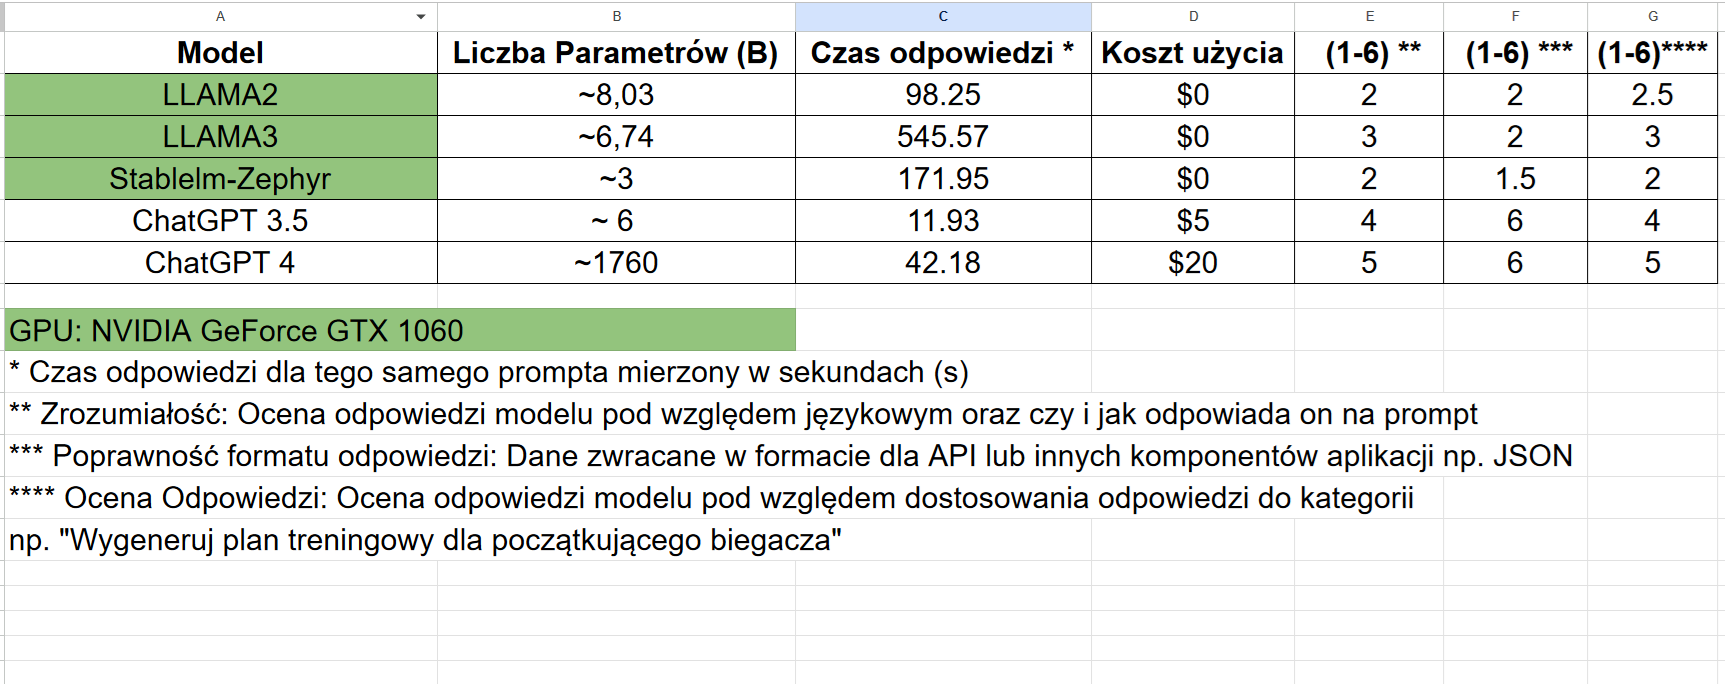
\includegraphics[width=1\textwidth]{Obrazy/llms_benchmark.png}
    \caption{Benchmark modeli LLM}
    \label{fig:my_label}
\end{figure}

Ranking modeli został przeprowadzony na środowisku lokalnym\linebreak z kartą graficzną NVIDIA GeForce GTX 1060. Na podanej wyżej tabeli zaznaczono nazwy modeli kolorem zielonym, które są modelami open source i można je skonfigurować do pracy na środowisku lokalnym. W rankingu uwzględniono liczbę parametrów danego modelu wyrażoną w miliardach. Następnie czas odpowiedzi na ten sam prompt dotyczący prośby o wygenerowanie planu treningowego dla użytkownika aplikacji. Dołączone zostały również koszty jakie trzeba ponieść aby dany model językowy mógł funkcjonować, pomijając koszty winikające z opłat energii elektrycznej i innych czynników zewnętrznych. Szybko można zauważyć dość oczywistą zależność, że płatne modele Chat GPT odpowiadają szybciej niż te na lokalnej maszynie. Dedykowane środowiska oraz konfiguracje zapewnione przez firmę OpenAI powodują, że model językowy odpowiada w sposób niemal natychmiastowy, nie trzeba oczekiwać na kolejne generowane słowa długo. Czas jest jednym z kluczowych aspektów podczas budowania aplikacji, użytkownik nie powinien być zmuszony do długiego oczekiwania na efekt końcowy. Żeby modele lokalne nie odbiegały prędkością odpowiedzi swojemu płatnemu odpowiednikowi, należałoby zainwestować w lepszą kartę graficzną bądź skorzystać \linebreak z dedykowanego chmurowego rozwiązania z profesjonalnym chipem, zoptymalizowanym pod sztuczną inteligencję. Niestety budżet naszego projektu nie był na tyle duży, aby podjąć się takiego przedsięwzięcia.
\\

\noindent Modele zostały ocenione w 6 stopniowej skali oceniania w kategoriach:
\begin{enumerate}
    \item zrozumiałość zwróconego tekstu
    \item poprawność formatu odpowiedzi
    \item ocena odpowiedzi pod względem umiejętności dopasowania generowanych danych dla użytkownika końcowego
\end{enumerate}

\paragraph{} Tutaj modele OpenAI ponownie dominują nad swoją konkurencją. Nie tylko lepiej dostosowywują się do zadanego prompta, ale też łatwiej dodać ich efekty operacji do finalnej aplikacji.
Plany oraz zadania były znacznie wyższej jakości niż darmowych odpowiedników. Przyglądając się liczbie parametrów można założyć tezę, że model firmy Meta z  ok. 8B parametrów poradzi sobie lepiej niż ChatGPT, jednak znany chatbot poradził sobie lepiej z generowaniem treści.

\clearpage

\subsubsection{Analiza Wydajności Modeli}

Ważnym aspektem w projektowaniu aplikacji, której zawartość oraz treść jest generowana przez model sztucznej inteligencji jest wydajność. Przeprowadzono analizę porównawczą wydajności różnych modeli językowych w kontekście generowania treści na zadany temat. Wykorzystano to samo pytanie, jak i rozszerzonego kontekstu, pozwalający na dokładniejszą ocenę, jak modele radzą sobie z różnymi typami zapytań.

Program ten realizuje proces generowania planu treningowego dla amatora, który chce przebiec maraton w ciągu roku, oraz analizuje wydajność różnych modeli językowych użytych do tego celu. W tym celu wykorzystuje pytanie dotyczące stworzenia planu treningowego oraz kontekst, który informuje, że zadaniem modelu jest dostarczenie treści do aplikacji internetowej.

\begin{lstlisting}[language=python, caption=Krok generowania planu treningowego]
# question
q = '''
Imagine that you are amateur person that wants to run 
a marathon in one year. This person about 10 hours to 
practice during week. Create plan that will last one year. 
Today is 23 April 2024 Create goal for every month. 
Include full name of every month and full date in format 
dd-mm-yyyy. Try to explain every task as precisely as you can.
'''

# context
cntx = '''
Your job will be play a role as content provider 
to the web application. You will get a task 
description and your job is to prepare plan for certain goal
'''

# models
models = ['llama2','llama3','stablelm-zephyr']
\end{lstlisting}

Program testuje trzy modele językowe: llama2, llama3 oraz stablelm-zephyr. Dla każdego z tych modeli najpierw generuje odpowiedzi na podstawie samego pytania, a następnie na podstawie pytania rozszerzonego o kontekst. Czas trwania generowania odpowiedzi jest mierzony i zapisywany.

Wyniki generowania treści, w tym metryki wydajności, są przechowywane i analizowane za pomocą biblioteki pandas. Metryki te obejmują całkowity czas trwania, czas ładowania, liczbę ocenianych podpowiedzi, liczbę ocen, czas oceny podpowiedzi oraz czas oceny. Program oblicza również dodatkowe parametry, takie jak czas obliczeń, szybkość przetwarzania podpowiedzi oraz szybkość ocen.

Dane te są następnie wizualizowane za pomocą wykresów słupkowych, które przedstawiają czas ładowania, szybkość przetwarzania podpowiedzi oraz szybkość ocen dla każdego modelu. Wykresy te pozwalają na łatwe porównanie wydajności różnych modeli językowych i oceny ich przydatności do określonego zadania.

Program ma na celu nie tylko wygenerowanie planu treningowego, ale także przeprowadzenie analizy porównawczej wydajności różnych modeli językowych w kontekście generowania treści na zadany temat. Wykorzystanie zarówno samego pytania, jak i rozszerzonego kontekstu, pozwala na dokładniejszą ocenę, jak modele radzą sobie z różnymi typami zapytań. Poniżej przedstawiono wyniki przeprowadzone lokalnie na karcie graficznej NVIDIA GTX 1060.

\begin{figure}[H]
    \centering
    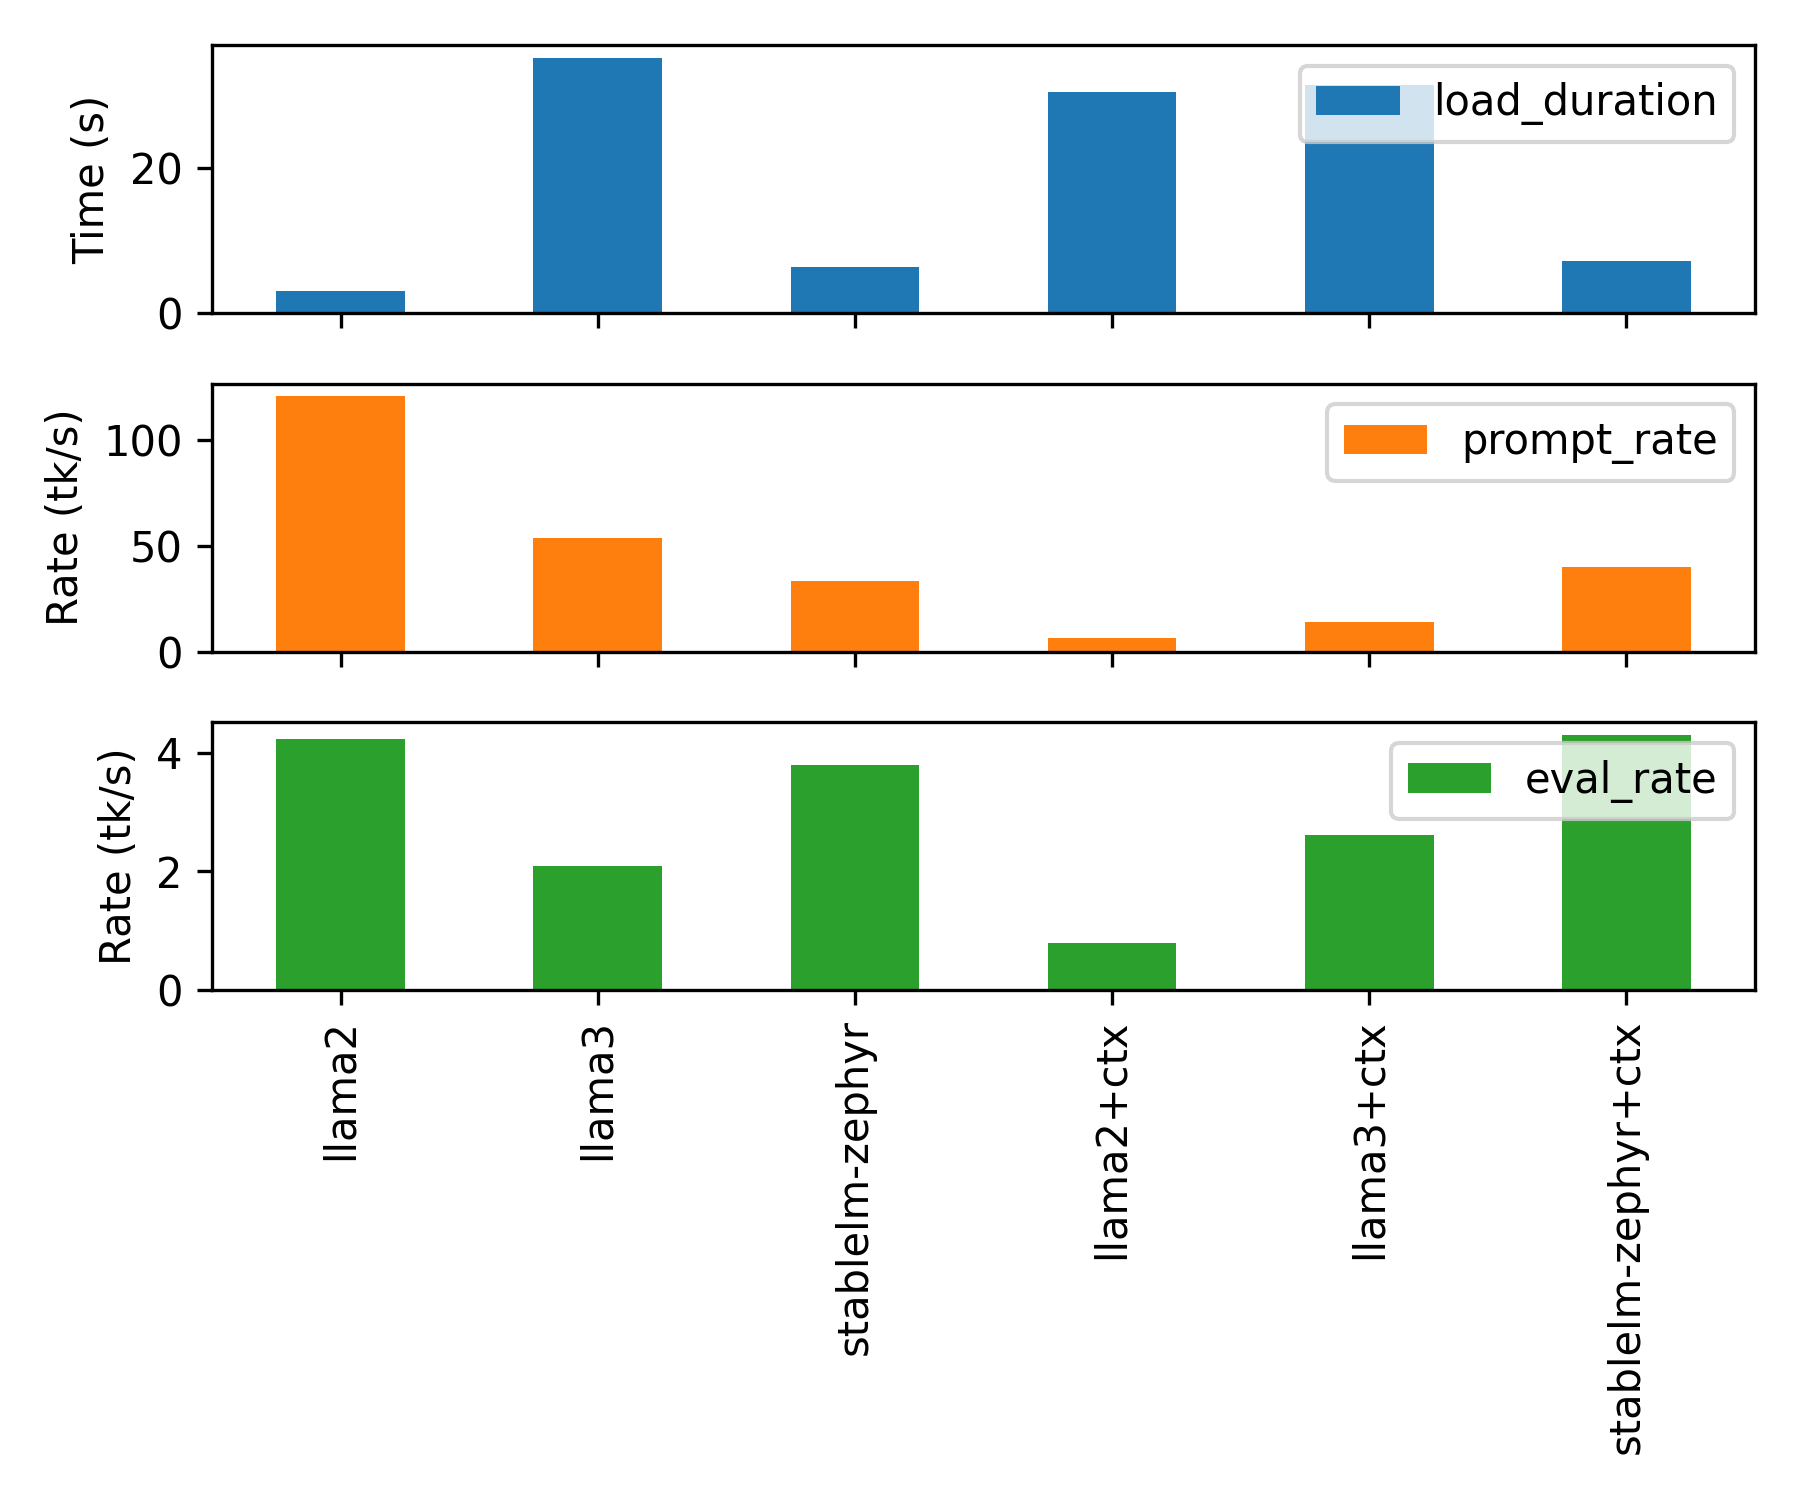
\includegraphics[width=1\textwidth]{Obrazy/results.png}
    \caption{Analiza Wydajności Modeli}
    \label{fig:my_label}
\end{figure}

Analizując wyniki przetwarzania trzech modeli językowych razem bez konstektsu oraz z kontekstem (ctx): llama2, llama3, stablelm-zephyr, llama2+ctx, llama3+ctx i stablelm-zephyr+ctx, można zauważyć znaczne różnice w ich wydajności i efektywności.


\noindent Zmierzono trzy kluczowe atrybuty:
\begin{enumerate}
    \item calc\_duration: Czas obliczeń jako różnicę między całkowitym czasem trwania a czasem ładowania.
    \item prompt\_rate: Szybkość przetwarzania podpowiedzi, czyli liczba ocenianych podpowiedzi na jednostkę czasu (tk/s).
    \item eval\_rate: Szybkość ocen, czyli liczba ocen na jednostkę czasu (tk/s).
\end{enumerate}

Model stablelm-zephyr+ctx osiągnął najkrótszy czas przetwarzania wynoszący 184.62 sekundy, co czyni go najbardziej efektywnym pod względem całkowitego czasu trwania. W przeciwieństwie do niego, model llama2+ctx miał najdłuższy czas przetwarzania, wynoszący aż 2160.26 sekund, co może wskazywać na problemy z optymalizacją lub nadmierne obciążenie obliczeniowe tego modelu.

Czas ładowania modeli również wykazuje różnice. Model llama2 charakteryzuje się najkrótszym czasem ładowania wynoszącym 3.01 sekundy, podczas gdy model llama3 potrzebował na to 35.13 sekund, co jest najdłuższym czasem ładowania spośród wszystkich analizowanych modeli.

Pod względem liczby ocenianych podpowiedzi (prompt\_eval\_count), model llama2+ctx ocenił najwięcej, bo aż 139 podpowiedzi, natomiast model llama3 ocenił ich najmniej, bo jedynie 87. Liczba ocen przeprowadzonych przez modele również była zróżnicowana. Najwięcej ocen, bo aż 1668, przeprowadził model llama2+ctx, a najmniej – 517 – model llama3+ctx.

Czas oceny podpowiedzi (prompt\_eval\_duration) był najdłuższy dla modelu llama2+ctx, wynosząc 21.32 sekundy, co kontrastuje z najkrótszym czasem oceny podpowiedzi modelu llama2, który wynosił zaledwie 0.88 sekund. Podobne różnice zauważalne są w czasie oceny (eval\_duration), gdzie model llama2+ctx potrzebował 2108.58 sekundy, a model stablelm-zephyr+ctx jedynie 174.21 sekundy.

Czas obliczeń (calc\_duration) dla modeli również wykazywał znaczne różnice. Najdłuższy czas obliczeń miał model llama2+ctx, wynosząc 2129.91 sekundy, podczas gdy model stablelm-zephyr+ctx osiągnął najkrótszy czas obliczeń, wynoszący 177.46 sekundy.

Analizując szybkość przetwarzania podpowiedzi (prompt\_rate), model llama2 osiągnął najwyższą szybkość wynoszącą 120.38, co kontrastuje z najniższą szybkością modelu llama2+ctx, która wynosiła 6.52. Szybkość oceny (eval\_rate) była najwyższa w przypadku modelu stablelm-zephyr+ctx, wynosząc 4.30, a najniższa u modelu llama2+ctx, wynosząc jedynie 0.79.

\begin{figure}[H]
    \centering
    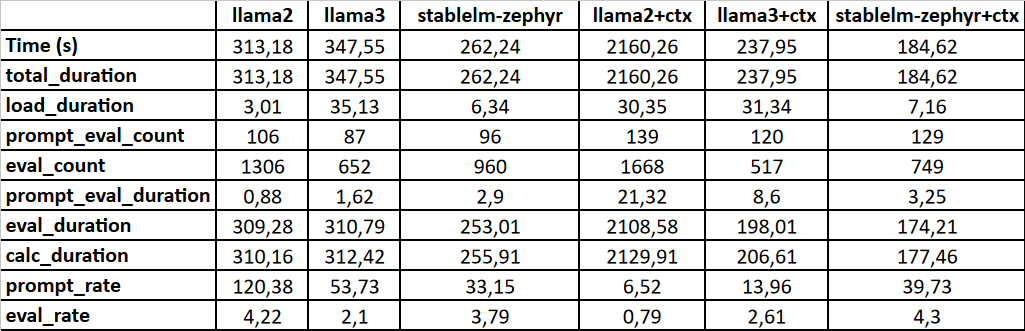
\includegraphics[width=1\textwidth]{Obrazy/benchmark_excel.png}
    \caption{Podsumowanie wyników}
    \label{fig:my_label}
\end{figure}

Warto pamiętać, że w komercyjnych i profesjonalnych warunkach wyniki wyglądałyby zupełnie inaczej. Do zapewnienia w aplikacji szybkiej analizy danych oraz czasu odpowiedzi potrzeba odpowiedniej mocy obliczeniowej, która często jest nie dostępna dla przeciętnego użytkownika. Kolejnym czynnikiem są parametry na których model był trenowany, im większa ilość parametrów tym czas odpowiedzi będzie dłuższy. Model taki jak zephyr miałby lepsze zastosowanie jako model odpowiedzialny np. za prostą komunikację z klientem, gdzie trzeba wygenerować prostą odpowiedź w jak najkrótszym czasie. Natomiast llama3 lepiej sprawdzi się do głębszej analizy danych.

\subsection{Platformy chmurowe}
Platformy chmurowe to zaawansowane systemy, które umożliwiają firmom i organizacjom dostęp do zasobów obliczeniowych przez Internet, bez konieczności posiadania i zarządzania własną infrastrukturą IT.

Platforma chmurowa to komponenty składające się z systemów operacyjnych, serwerów w centrum danych skonfigurowanych pod personalne potrzeby klientów. Umożliwiają one organizacjom wynajmowanie dostępu do zasobów obliczeniowych, takich jak serwery, bazy danych, magazyny danych, analityk, sieci wirtualnych. Model biznesowy dostawców usług chmurowych opiera się na zasadzie "pay as you go" (z .ang) płać za te zasoby, które zużyjesz.[20]

\noindent{\bf Usługi chmurowe możemy podzielić na trzy kluczowe rodzaje:}

\begin{enumerate}
    \item {\bf Chmura Publiczna:} Usługi świadczone przez zewnętrznych dostawców, dostępne dla wielu klientów przez Internet. Przykłady to Amazon Web Services (AWS), Google Cloud Platform, Microsoft Azure, Alibaba Cloud i IBM Cloud.
    \item {\bf  Chmura Prywatna:} Dedykowana dla jednej organizacji, może być zarządzana wewnętrznie lub przez zewnętrznego dostawcę. Oferuje większą kontrolę nad zasobami i bezpieczeństwem.
    \item {\bf Chmura Hybrydowa:} Chmura Hybrydowa: Kombinacja chmury publicznej i prywatnej, umożliwiająca przenoszenie danych i aplikacji między nimi, co zapewnia większą elastyczność i optymalizację infrastruktury.
\end{enumerate} 

\noindent{\bf Korzyści z Używania Platform Chmurowych:}
\begin{enumerate}
    \item {\bf Elastyczność:}  Możliwość szybkiego skalowania zasobów w górę lub w dół w zależności od potrzeb biznesowych, co pozwala uniknąć nadmiernego lub niedostatecznego przydziału zasobów obliczeniowych.
    \item {\bf Redukcja Kosztów:}  Eliminacja kosztów kapitałowych związanych z budową i utrzymaniem własnych centrów danych oraz płatność tylko za faktycznie używane zasoby.
    \item {\bf Wydajność:} Dostęp do dużej mocy obliczeniowej i magazynowej na żądanie, co pozwala unikać wąskich gardeł i zapewnia lepszą wydajność aplikacji.
    \item {\bf Szybkość Wdrożenia:} Możliwość szybkiego wdrażania technologii na całym świecie, co skraca czas wprowadzenia produktów na rynek.
    \item {\bf Zwiększona Produktywność:} Zespoły IT są zwolnione z zarządzania, utrzymania i aktualizacji sprzętu i oprogramowania na miejscu, co pozwala im skupić się na bardziej strategicznych zadaniach.
    \item {\bf Bezpieczeństwo:} Dostawcy chmurowi inwestują znaczne środki w technologie zabezpieczające, co często zapewnia wyższy poziom bezpieczeństwa niż w przypadku własnych centrów danych.
    \item {\bf Niezawodność:} Platformy chmurowe są bardziej odporne dzięki rozproszonej infrastrukturze, co zapewnia szybsze odzyskiwanie danych po awariach systemów.
    
\end{enumerate}
Platformy chmurowe odgrywają kluczową rolę w nowoczesnych strategiach IT, umożliwiając firmom szybkie i efektywne skalowanie swoich operacji oraz wprowadzanie innowacji.

\subsubsection{Opis platform}
Platformy chmurowe to zintegrowane zestawy technologii umożliwiające użytkownikom zdalne korzystanie z szerokiej gamy zasobów komputerowych przez Internet. Te cyfrowe ekosystemy oferują skalowalne rozwiązania IT, takie jak serwery, pamięć, bazy danych oraz oprogramowanie, wszystko dostępne jako usługa. Główne kategorie tych usług to: Infrastructure as a Service (IaaS), Platform as a Service (PaaS) oraz Software as a Service (SaaS).

Korzystanie z platform chmurowych przynosi wiele korzyści. Elastyczność i skalowalność pozwalają na szybkie dostosowywanie zasobów do aktualnych potrzeb, bez konieczności inwestycji w drogi sprzęt i infrastrukturę. Oszczędności kosztów wynikają z modelu opłat "pay as you go", co oznacza, że płaci się tylko za te zasoby, które są faktycznie wykorzystywane. Bezpieczeństwo danych jest również kluczowym aspektem, z zaawansowanymi rozwiązaniami chroniącymi przed utratą danych i cyberatakami [21].

\subsubsection{Wybór - Plaftorma Microsoft Azure}
Platforma Azure została wybrana do naszego projektu ze względu na to,że nasz zespół miał już doświadczenie zarówno prywatne jak i komercyjne w tej technologii. Kolejnym atutem rozwiązania firmy z Redmond, jest bogata oferta serwisów oraz technologii potrzebnych do zbudowania do aplikacji opartej o architekturę mikroserwisów.
W tym kontekście, Azure okazuje się być idealną platformą do rozwijania mikroserwisów dzięki usługom takim jak Azure Kubernetes Service, który upraszcza zarządzanie kontenerami, oraz Azure Container Instances. Platforma oferuje również integrację z narzędziami deweloperskimi oraz CI/CD.[22][23]

\clearpage

\subsection{Wymagania funkcjonalne}

\subsubsection{Opis funkcjonalności systemu}

\noindent Aplikacja ma posiadać następujące funkcjonalności systemu:
\begin{enumerate}
    \item[*] {\bf Rejestracja użytkownika} - polega na utworzeniu konta użytkownika poprzez podanie adresu e-mail, nazwy i hasła.
    \item[*] {\bf Logowanie użytkownika} - umożliwia zalogowanie się do aplikacji za pomocą adresu e-mail i hasła.
    \item[*] {\bf Tworzenie celów} - pozwala użytkownikowi na definiowanie nowych celów do osiągnięcia.
    \item[*] {\bf Generowanie planów} - wykorzystuje modele LLM do generowania planów działania dla zdefiniowanych celów.
    \item[*] {\bf Wyświetlanie listy zadań} - prezentuje użytkownikowi listę zadań do wykonania w celu osiągnięcia zamierzonego celu.
    \item[*] {\bf Zarządzanie zadaniami} - umożliwia użytkownikowi oznaczanie zadań jako ukończone lub nieukończone.
    \item[*] {\bf Przyznawanie osiągnięć} - moduł, który przyznaje użytkownikom odznaki za realizację określonej liczby celów i zadań, motywując ich do dalszego działania. Użytkownicy mogą zdobywać różne odznaki, które są widoczne na ich profilach.
    \item[*] {\bf Integracja z modelami LLM} - zapewnia komunikację z wybranymi modelami LLM w celu generowania planów działania.
    \item[*] {\bf Zabezpieczone strony} - chroni dostęp do określonych stron aplikacji, wymagając uprzedniego zalogowania.
\end{enumerate}

\clearpage

\subsubsection{Diagram przypadków użycia}

\begin{figure}[H]
    \centering
    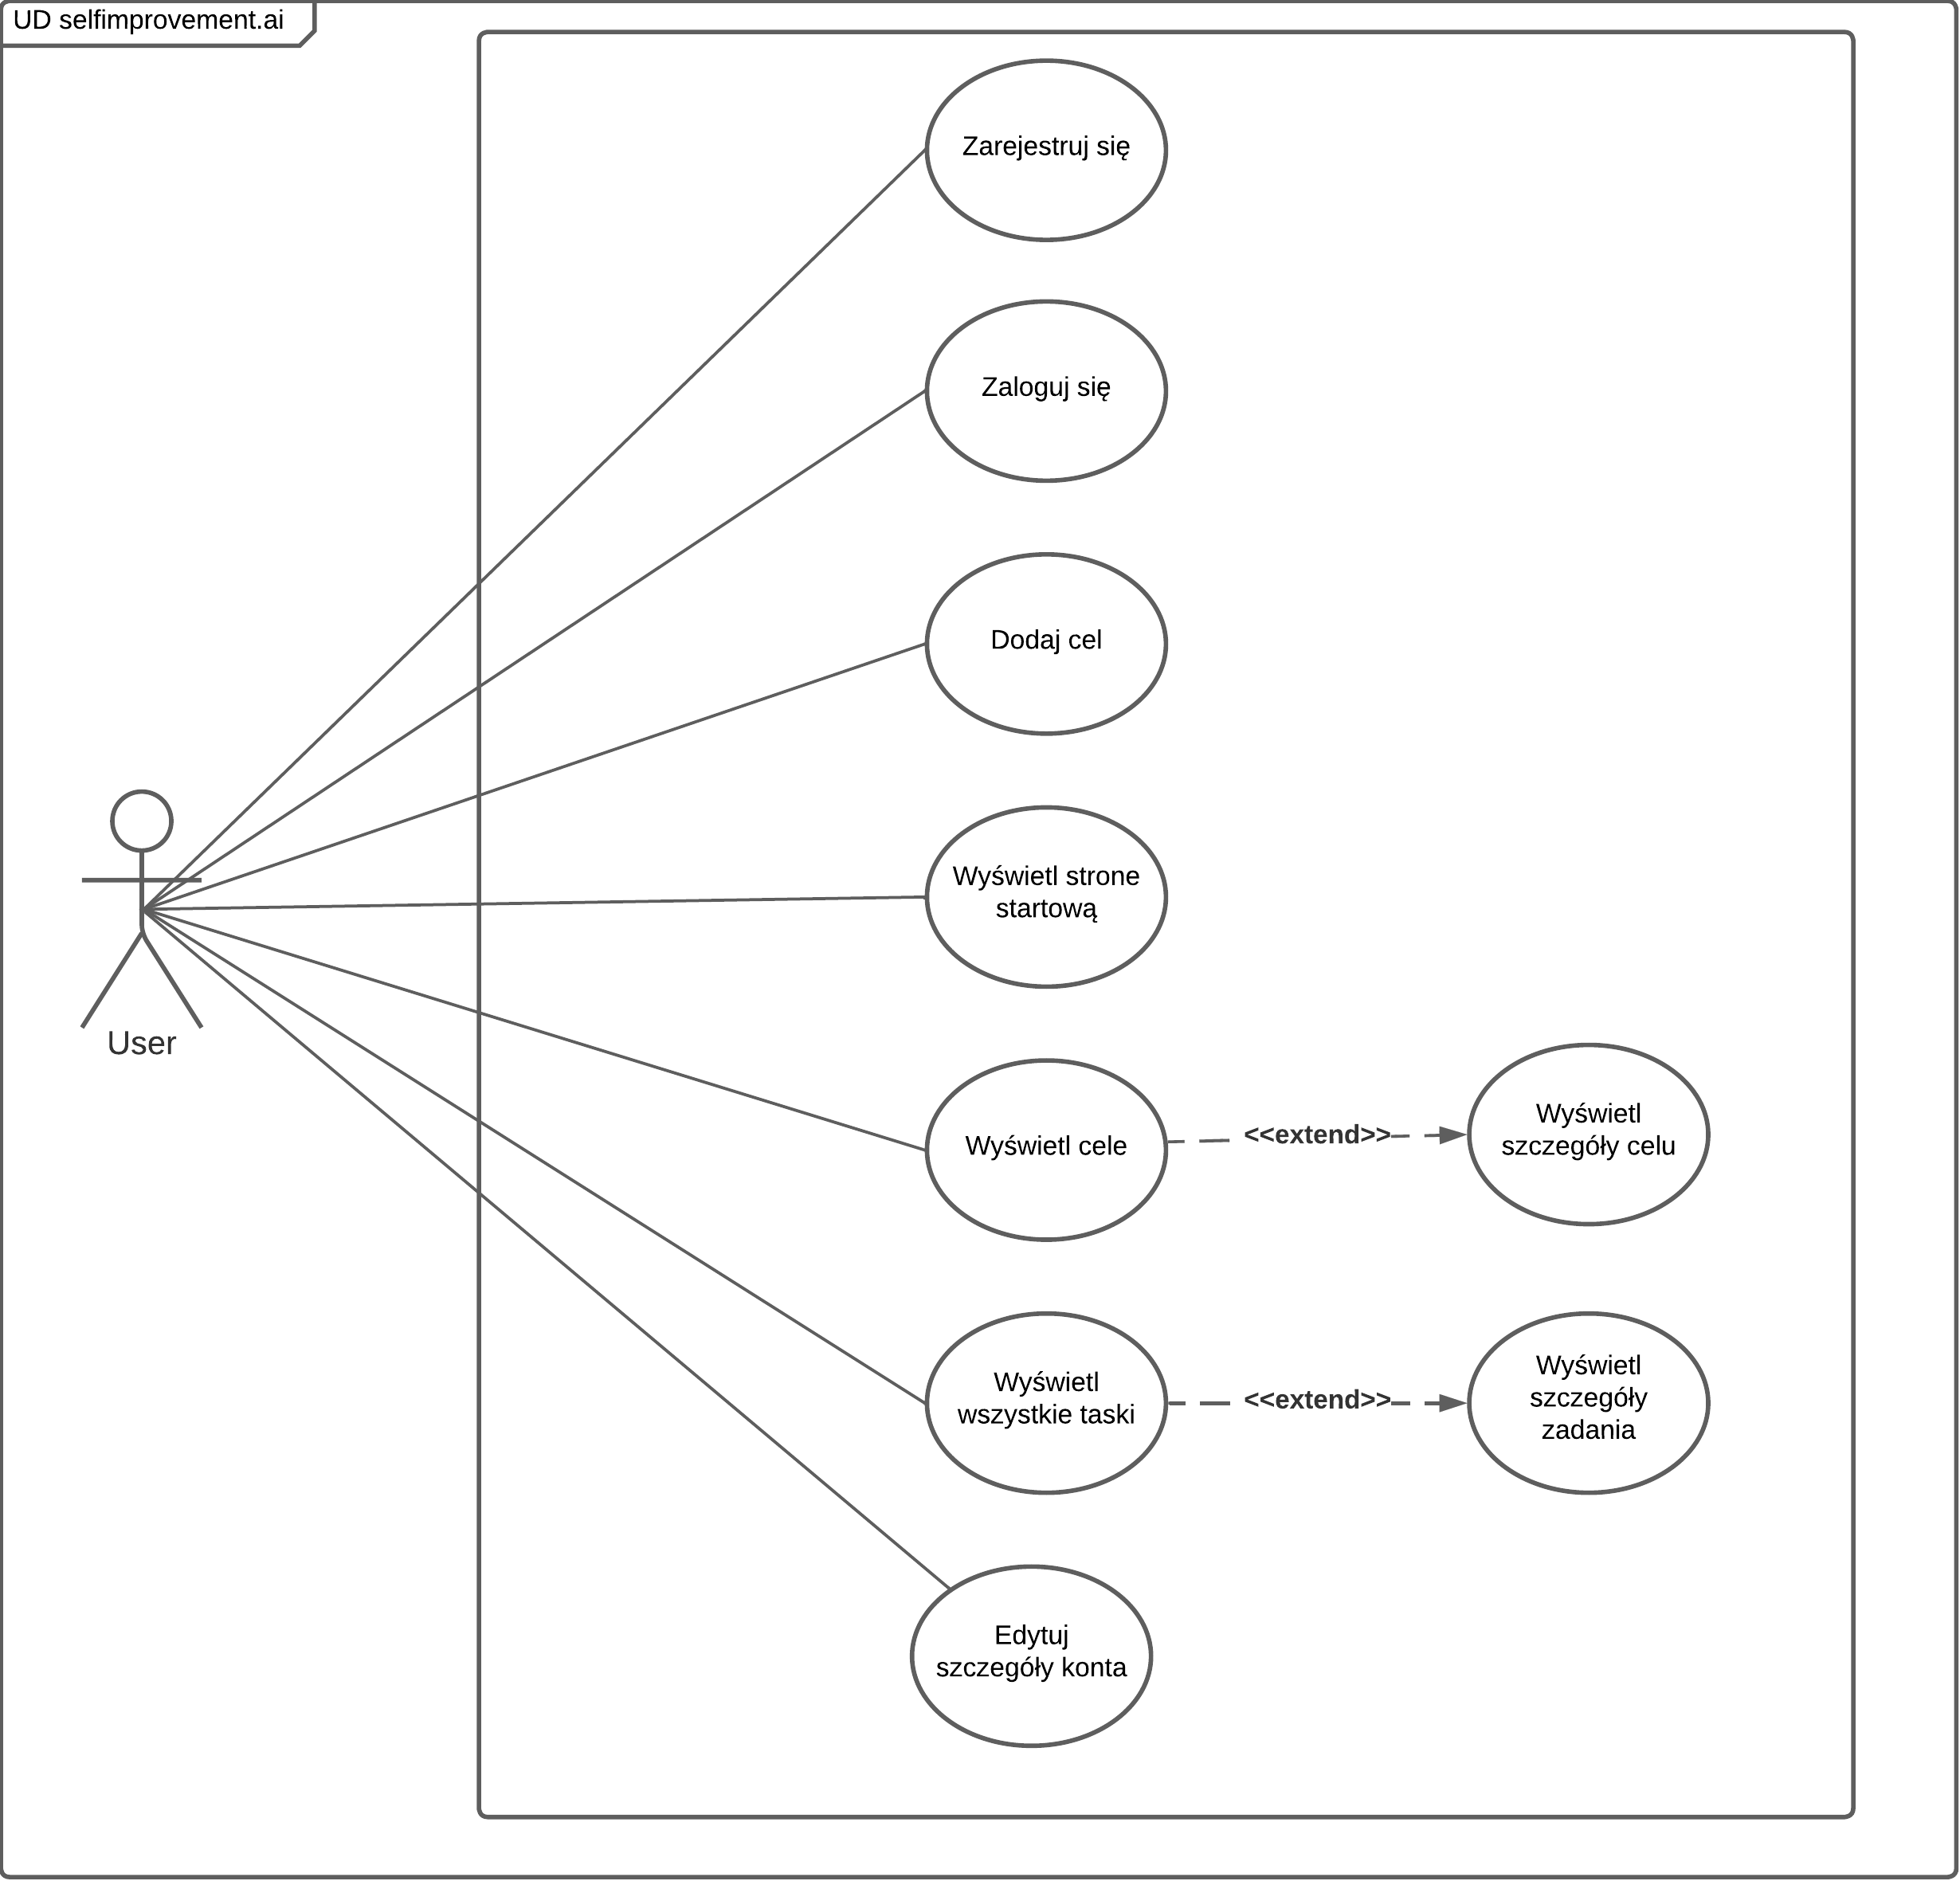
\includegraphics[width=0.9\textwidth]{Obrazy/diagrams/use_case_diagram.png}
    \caption{Diagram przypadków użycia}
    \label{fig:my_label}
\end{figure}

Diagram przypadków użycia przedstawia interakcje użytkownika \linebreak z systemem oraz ilustruje główne funkcjonalności oferowane przez aplikację. W kontekście naszej aplikacji, która wspiera użytkowników w osiąganiu różnych celów za pomocą generowania planów przez modele LLM, diagram przypadków użycia zawiera kilka kluczowych przypadków użycia oraz aktorów.

\begin{itemize}
    \item \textbf{Aktorzy}:
    \begin{itemize}
        \item[*] \textbf{Użytkownik}: Osoba korzystająca z aplikacji, która może rejestrować się, logować, dodawać cele, przeglądać zadania i cele oraz zarządzać swoimi informacjami.
    \end{itemize}
    \clearpage

    \item \textbf{Przypadki użycia}:
    \begin{itemize}
        \item[*] \textbf{Rejestracja użytkownika}: Proces tworzenia nowego konta w systemie.
        \item[*] \textbf{Logowanie użytkownika}: Proces uwierzytelniania istniejącego użytkownika.
        \item[*] \textbf{Dodawanie celu}: Umożliwia użytkownikowi dodanie nowego celu do aplikacji.
        \item[*] \textbf{Wyświetlanie strony startowej}: Pokazuje użytkownikowi główny widok aplikacji po zalogowaniu.
        \item[*] \textbf{Wyświetlanie celów}: Wyświetla listę wszystkich celów użytkownika.
        \item[*] \textbf{Wyświetlanie szczegółów celu}: Pokazuje szczegółowe informacje dotyczące wybranego celu.
        \item[*] \textbf{Wyświetlanie wszystkich zadań}: Umożliwia przeglądanie wszystkich zadań użytkownika.
        \item[*] \textbf{Wyświetlanie szczegółów zadania}: Pokazuje szczegółowe informacje dotyczące wybranego zadania.
        \item[*] \textbf{Edycja szczegółów konta}: Umożliwia użytkownikowi zmianę swoich danych profilowych.
        \item[*] \textbf{Przyznawanie osiągnięć}: System przyznaje użytkownikowi odznaki za osiągnięcie określonych celów lub zadań.
    \end{itemize}
\end{itemize}

Diagram przypadków użycia pomaga zrozumieć, jakie funkcjonalności są dostępne w systemie i w jaki sposób użytkownicy mogą z nimi wchodzić w interakcję. Jest to kluczowe narzędzie w procesie projektowania i rozwijania aplikacji, które zapewnia klarowność i precyzję w definiowaniu wymagań systemu.

\subsubsection{Scenariusze przypadków użycia}

Scenariusze przypadków użycia opisują interakcję między użytkownikiem a systemem w kontekście osiągania określonych celów. Każdy scenariusz przedstawia sekwencję kroków, które użytkownik wykonuje, aby zrealizować daną funkcjonalność systemu. Scenariusze te pomagają w zrozumieniu wymagań użytkownika oraz w identyfikacji funkcjonalności, które system musi zapewnić. Stanowią one podstawę do projektowania i implementacji systemu, zapewniając klarowność i precyzję w definiowaniu oczekiwań wobec systemu.
\\

{\noindent \bf{\small 1. Rejestracja użytkownika\par}}
\vspace{0.5cm}
{\noindent \bf Kontekst użycia: } Rejestracja użytkownika w systemie\\
{\bf Poziom: } Cel użytkownika\\
{\bf Aktor główny: } Użytkownik\\
{\bf Warunek początkowy: } W aplikacji (bazie danych) użytkownik nie posiada konta\\
{\bf Gwarancja powodzenia: } W aplikacji (bazie danych) został zarejestrowany użytkownik\\
{\bf Wyzwalacz: } Użytkownik\\
{\bf Główny scenariusz powodzenia: }
\begin{center}
    \begin{enumerate}
        \item Użytkownik (aktor) uruchamia przypadek użycia
        \item Aktor wypełnia formularz rejestracyjny i klika przycisk rejestracji
        \item System zapisuje dane użytkownika i tworzy nowe konto
        \item Wyświetla się strona z panelem użytkownika
        \item Aplikacja kończy przypadek użycia
    \end{enumerate}
\end{center}
{\noindent \bf Rozszerzenia: }
\begin{center}
    \begin{description}
        \item{2a.} Podany adres e-mail jest już zarejestrowany, rejestracja nie powiodła się
    \end{description}
\end{center}

\noindent\rule{14cm}{0.1pt} % długość i grubość linii

{\noindent \bf{\small 2. Logowanie użytkownika\par}}
\vspace{0.5cm}
{\noindent \bf Kontekst użycia: } Logowanie użytkownika do systemu\\
{\bf Poziom: } Cel użytkownika\\
{\bf Aktor główny: } Użytkownik\\
{\bf Warunek początkowy: } W aplikacji (bazie danych) użytkownik posiada konto\\
{\bf Gwarancja powodzenia: } W aplikacji użytkownik został zalogowany\\
{\bf Wyzwalacz: } Użytkownik\\
{\bf Główny scenariusz powodzenia: }
\begin{center}
    \begin{enumerate}
        \item Użytkownik (aktor) uruchamia przypadek użycia
        \item Aktor wypełnia formularz logowania i klika przycisk logowania
        \item System weryfikuje dane i loguje użytkownika
        \item Wyświetla się strona z panelem użytkownika
        \item Aplikacja kończy przypadek użycia
    \end{enumerate}
\end{center}
{\noindent \bf Rozszerzenia: }
\begin{center}
    \begin{description}
        \item{2a.} Podany adres e-mail lub hasło jest nieprawidłowe, logowanie nie powiodło się
    \end{description}
\end{center}

\noindent\rule{14cm}{0.1pt} % długość i grubość linii

{\noindent \bf{\small 3. Dodaj cel\par}}
\vspace{0.5cm}
{\noindent \bf Kontekst użycia: } Dodawanie nowego celu przez użytkownika\\
{\bf Poziom: } Cel użytkownika\\
{\bf Aktor główny: } Użytkownik\\
{\bf Warunek początkowy: } Użytkownik jest zalogowany w systemie\\
{\bf Gwarancja powodzenia: } Nowy cel został zapisany w systemie\\
{\bf Wyzwalacz: } Użytkownik\\
{\bf Główny scenariusz powodzenia: }
\begin{center}
    \begin{enumerate}
        \item Użytkownik (aktor) uruchamia przypadek użycia
        \item Aktor wypełnia formularz dodawania celu i klika przycisk zapisu
        \item System zapisuje nowy cel
        \item Wyświetla się widok szczegółowy celu z nowo dodanymi zadaniami
        \item Aplikacja kończy przypadek użycia
    \end{enumerate}
\end{center}
{\noindent \bf Rozszerzenia: }
\begin{center}
    \begin{description}
        \item{2a.} Formularz zawiera nieprawidłowe dane, cel nie został zapisany
    \end{description}
\end{center}

\noindent\rule{14cm}{0.1pt} % długość i grubość linii

{\noindent \bf{\small 4. Wyświetl stronę startową\par}}
\vspace{0.5cm}
{\noindent \bf Kontekst użycia: } Wyświetlanie strony startowej aplikacji\\
{\bf Poziom: } Cel użytkownika\\
{\bf Aktor główny: } Użytkownik\\
{\bf Warunek początkowy: } Użytkownik jest zalogowany w systemie\\
{\bf Gwarancja powodzenia: } Strona startowa została poprawnie wyświetlona\\
{\bf Wyzwalacz: } Użytkownik\\
{\bf Główny scenariusz powodzenia: }
\begin{center}
    \begin{enumerate}
        \item Użytkownik (aktor) uruchamia przypadek użycia
        \item System ładuje i wyświetla stronę startową
        \item Aplikacja kończy przypadek użycia
    \end{enumerate}
\end{center}

\noindent\rule{14cm}{0.1pt} % długość i grubość linii

{\noindent \bf{\small 5. Wyświetl cele\par}}
\vspace{0.5cm}
{\noindent \bf Kontekst użycia: } Wyświetlanie listy celów użytkownika\\
{\bf Poziom: } Cel użytkownika\\
{\bf Aktor główny: } Użytkownik\\
{\bf Warunek początkowy: } Użytkownik jest zalogowany w systemie\\
{\bf Gwarancja powodzenia: } Lista celów została poprawnie wyświetlona\\
{\bf Wyzwalacz: } Użytkownik\\
{\bf Główny scenariusz powodzenia: }
\begin{center}
    \begin{enumerate}
        \item Użytkownik (aktor) uruchamia przypadek użycia
        \item System ładuje i wyświetla listę celów użytkownika
        \item Aplikacja kończy przypadek użycia
    \end{enumerate}
\end{center}

\noindent\rule{14cm}{0.1pt} % długość i grubość linii

{\noindent \bf{\small 6. Wyświetl szczegóły celu\par}}
\vspace{0.5cm}
{\noindent \bf Kontekst użycia: } Wyświetlanie szczegółów wybranego celu\\
{\bf Poziom: } Cel użytkownika\\
{\bf Aktor główny: } Użytkownik\\
{\bf Warunek początkowy: } Użytkownik jest zalogowany w systemie, posiada zapisane cele\\
{\bf Gwarancja powodzenia: } Szczegóły celu zostały poprawnie wyświetlone\\
{\bf Wyzwalacz: } Użytkownik\\
{\bf Główny scenariusz powodzenia: }
\begin{center}
    \begin{enumerate}
        \item Użytkownik (aktor) uruchamia przypadek użycia
        \item System ładuje i wyświetla szczegóły wybranego celu
        \item Aplikacja kończy przypadek użycia
    \end{enumerate}
\end{center}

\noindent\rule{14cm}{0.1pt} % długość i grubość linii

{\noindent \bf{\small 7. Wyświetl wszystkie zadania\par}}
\vspace{0.5cm}
{\noindent \bf Kontekst użycia: } Wyświetlanie listy wszystkich zadań\\
{\bf Poziom: } Cel użytkownika\\
{\bf Aktor główny: } Użytkownik\\
{\bf Warunek początkowy: } Użytkownik jest zalogowany w systemie\\
{\bf Gwarancja powodzenia: } Lista zadań została poprawnie wyświetlona\\
{\bf Wyzwalacz: } Użytkownik\\
{\bf Główny scenariusz powodzenia: }
\begin{center}
    \begin{enumerate}
        \item Użytkownik (aktor) uruchamia przypadek użycia
        \item System ładuje i wyświetla listę wszystkich zadań
        \item Aplikacja kończy przypadek użycia
    \end{enumerate}
\end{center}

\noindent\rule{14cm}{0.1pt} % długość i grubość linii

{\noindent \bf{\small 8. Wyświetl szczegóły zadania\par}}
\vspace{0.5cm}
{\noindent \bf Kontekst użycia: } Wyświetlanie szczegółów wybranego zadania\\
{\bf Poziom: } Cel użytkownika\\
{\bf Aktor główny: } Użytkownik\\
{\bf Warunek początkowy: } Użytkownik jest zalogowany w systemie, posiada zapisane zadania\\
{\bf Gwarancja powodzenia: } Szczegóły zadania zostały poprawnie wyświetlone\\
{\bf Wyzwalacz: } Użytkownik\\
{\bf Główny scenariusz powodzenia: }
\begin{center}
    \begin{enumerate}
        \item Użytkownik (aktor) uruchamia przypadek użycia
        \item System ładuje i wyświetla szczegóły wybranego zadania
        \item Aplikacja kończy przypadek użycia
    \end{enumerate}
\end{center}

\clearpage

{\noindent \bf{\small 9. Edytuj szczegóły konta\par}}
\vspace{0.5cm}
{\noindent \bf Kontekst użycia: } Edytowanie szczegółów konta użytkownika\\
{\bf Poziom: } Cel użytkownika\\
{\bf Aktor główny: } Użytkownik\\
{\bf Warunek początkowy: } Użytkownik jest zalogowany w systemie\\
{\bf Gwarancja powodzenia: } Szczegóły konta zostały poprawnie zaktualizowane\\
{\bf Wyzwalacz: } Użytkownik\\
{\bf Główny scenariusz powodzenia: }
\begin{enumerate}
    \item Użytkownik (aktor) uruchamia przypadek użycia
    \item System ładuje formularz edycji szczegółów konta
    \item Użytkownik wypełnia formularz i zapisuje zmiany
    \item System zapisuje zaktualizowane dane użytkownika
    \item Aplikacja kończy przypadek użycia
\end{enumerate}
{\noindent \bf Rozszerzenia: }
\begin{description}
    \item[4a.] Formularz zawiera nieprawidłowe dane, edycja nie powiodła się
\end{description}

\subsubsection{Sposób przechowywania danych}
Dane użytkowników są przechowywane w bazie danych PostgreSQL, co zapewnia efektywne zarządzanie dużymi zbiorami danych oraz wysoki poziom bezpieczeństwa. PostgreSQL, jako zaawansowany system zarządzania relacyjnymi bazami danych, oferuje szerokie możliwości skalowania i optymalizacji, co jest kluczowe przy obsłudze danych wrażliwych i osobowych.

\clearpage

\subsubsection{Diagramy}

{\noindent \bf Diagram aktywności dodania celu: }
\begin{figure}[H]
    \centering
    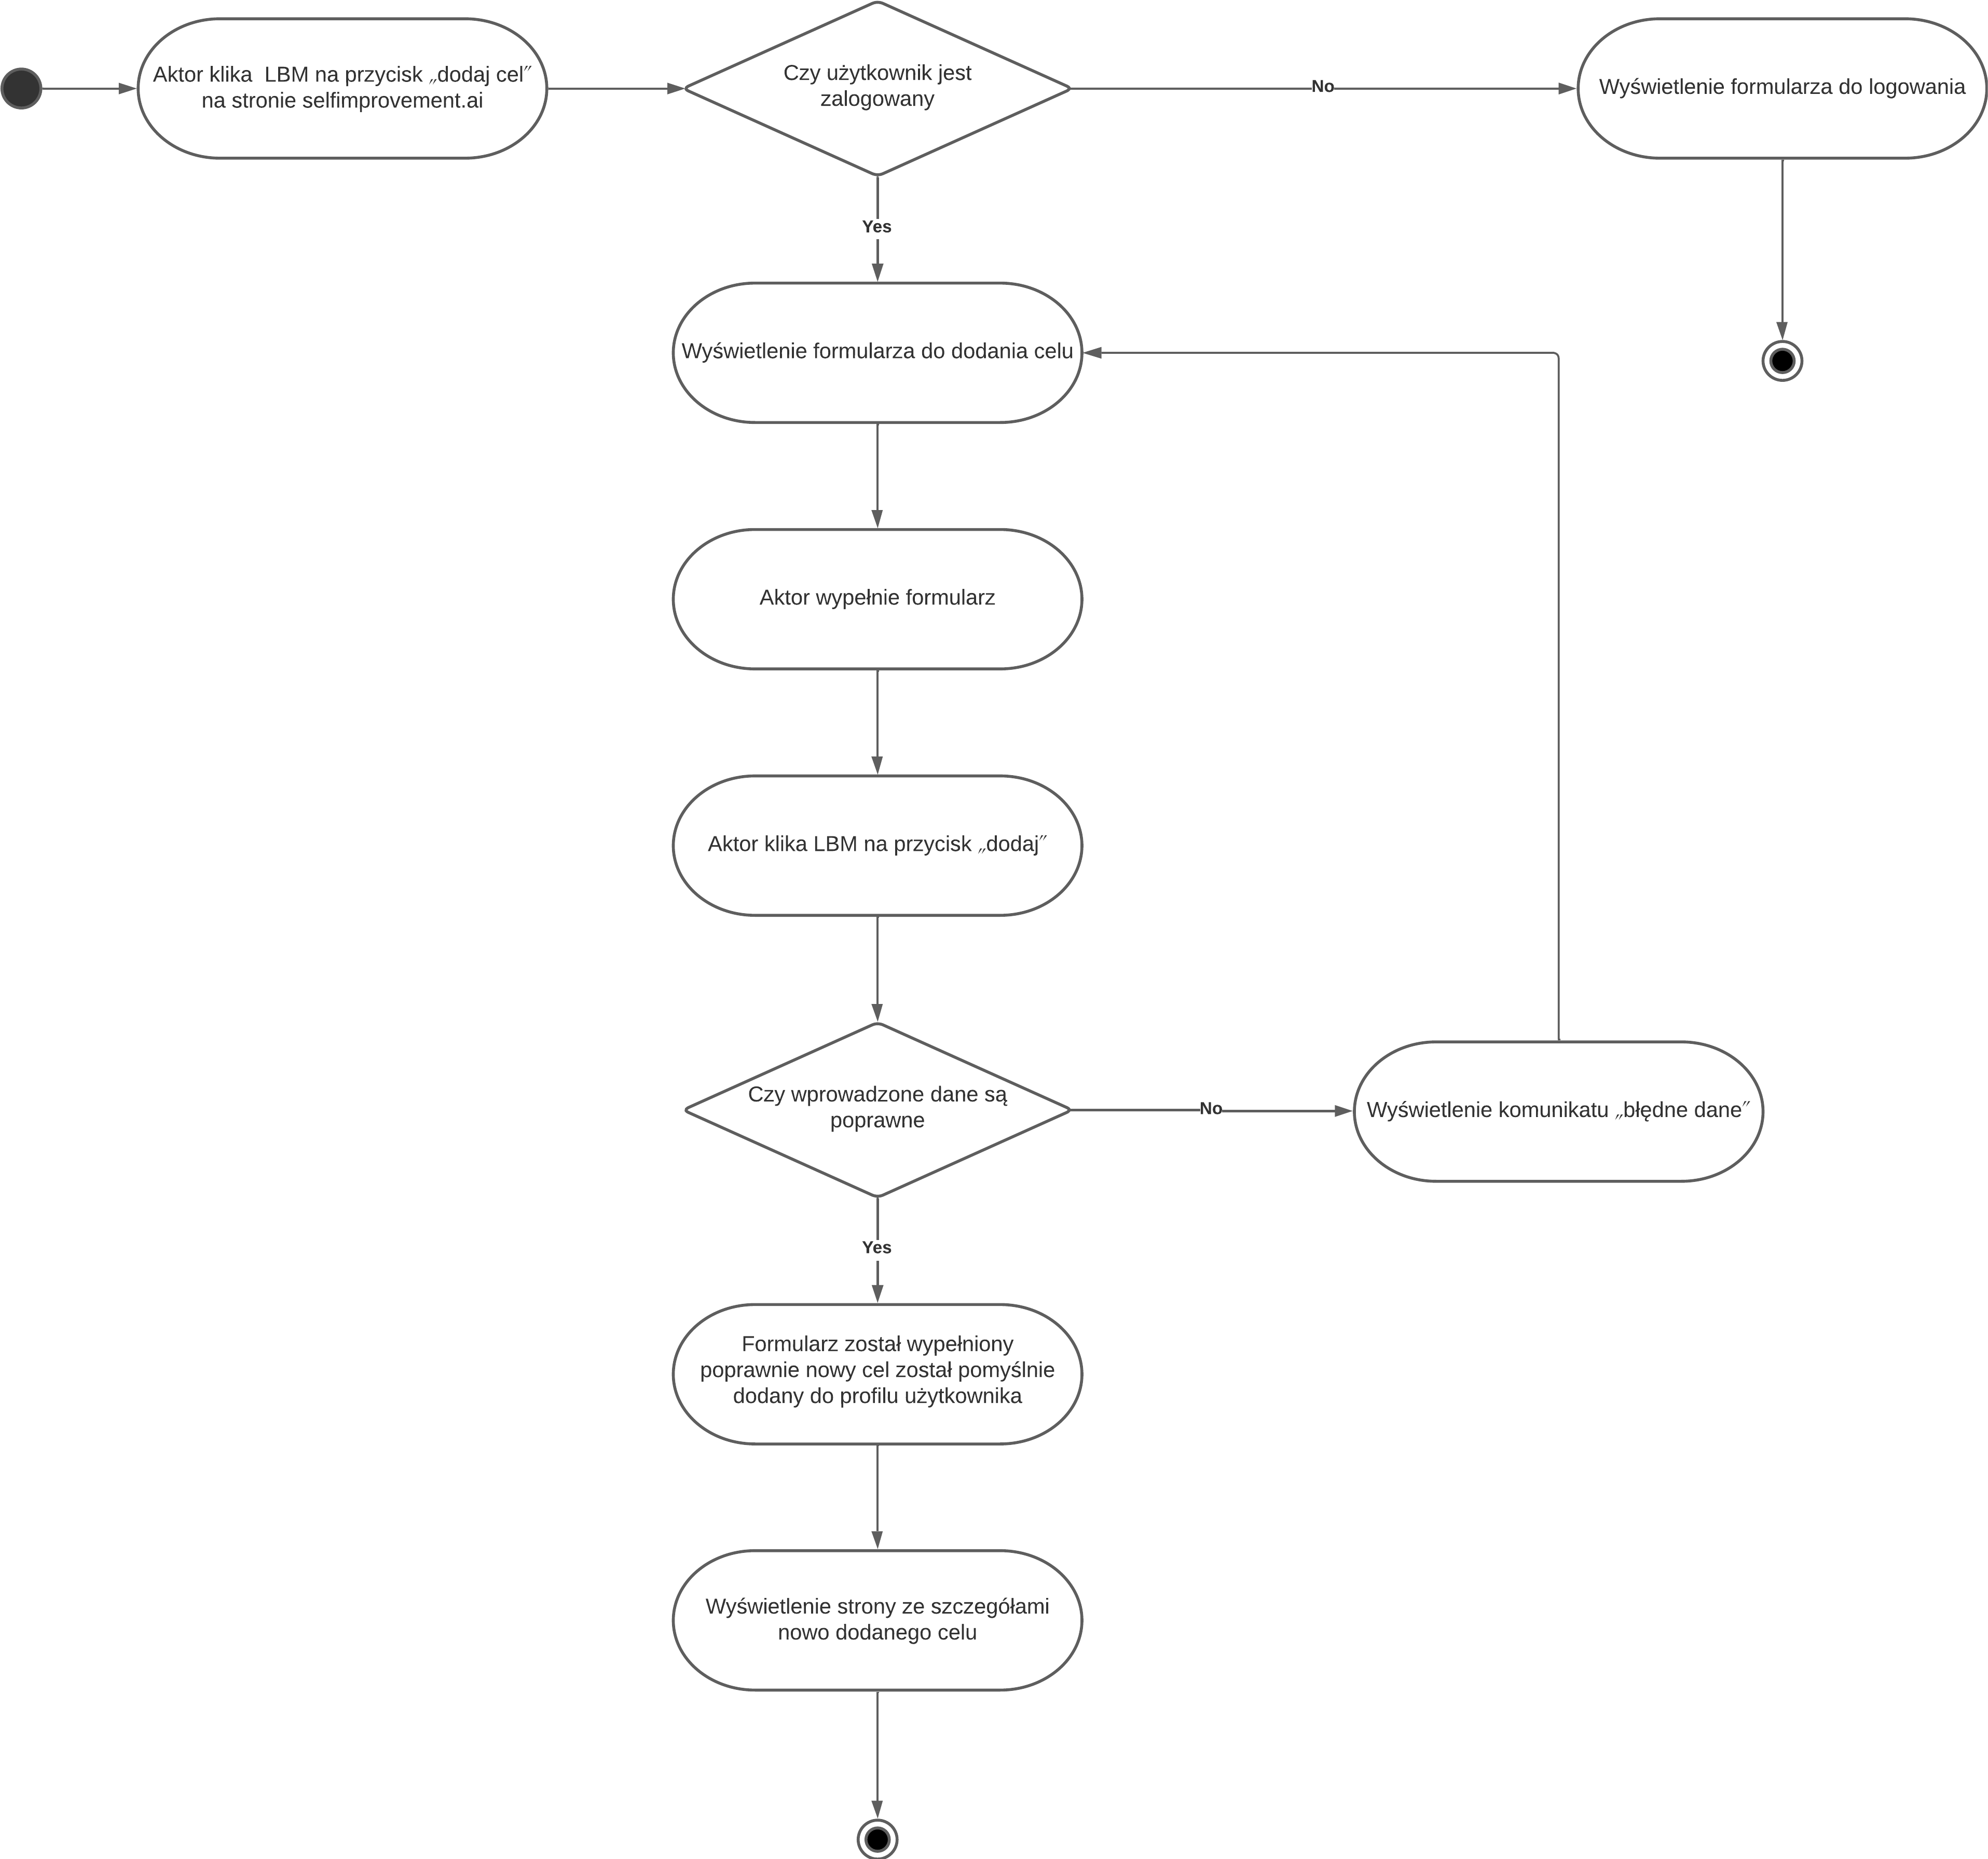
\includegraphics[width=1\textwidth]{Obrazy/diagrams/add_goal_activity_diagram.png}
    \caption{Diagram Aktywności dla przypadku dodanie celu}
    \label{fig:my_label}
\end{figure}

\noindent Powyższy diagram aktywności przedstawia cały proces dodawania celu od momentu rozpoczęcia do zakończenia. Uwzględnia on interakcje użytkownika z systemem, walidację danych, zapis do bazy danych oraz aktualizację interfejsu użytkownika. Jest to pomocne narzędzie do zrozumienia przepływu pracy oraz identyfikacji potencjalnych punktów poprawy w procesie.

\clearpage

\subsection{Wymagania niefunkcjonalne}
\begin{itemize}
    \item[*] W przypadku gdy użytkownik korzysta z komputera stacjonarnego lub urządzenia mobilnego aplikacja powinna działać na: Google Chrome(wersja 95 i wyżej), Firefox lub Opera. 
    \item[*] Aplikacja powinna poprawnie działać na środowisku chmurowym np. Azure. Rekomendowanym systemem operacyjnym jest 64 bitowy system GNU/Linux, ponieważ najlepiej jest on przystosowany do środowiska chmurowego. W przypadku użycia kontenerów zalecane jest utworzenie własnego repozytorium do przechowywania źródeł obrazów np. Azure Conainer Registry. Ddla każdego uruchomionego kontenera należy zapewnić minimum 1 rdzeń procesora oraz 2GB pamięci RAM. Dla optymalizacji działania aplikacji, wszystkie komponenty powinny się znajdować w tej samej lub bardzo do siebie zbliżonej lokalizacji, aby uniknąć zbędnych opóźnień.
    \item[*] Aplikacja uruchomiona na lokalnym środowisku powinna poprawnie działać na komputerze z zainstalowanym system operacyjnym wspierającym konteneryzację Docker oraz wirtualizację np. Ubuntu Linux lub Windows 10/11. Najlepiej używać procesora o architekturze "x86\_64/amd64" i posiadać minmalną ilość pamięci RAM wynoszącej 4GB.
\end{itemize}
\clearpage

\subsection{Opis prototypów}
Prototypy opracowane na etapie planowania całej aplikacji okazały się niezwykle pomocne w ustaleniu funkcjonalności oraz ogólnego zarysu aplikacji. Jednakże, po dokładnej analizie trendów dotyczących UX/UI oraz tematyki aplikacji, konieczne było wykonanie nowego aspektu wizualnego. Zmieniono kolorystykę oraz doprecyzowano wygląd poszczególnych komponentów, aby spełnić wymagania standardów UX/UI oraz zapewnić użytkownikom maksymalny komfort podczas korzystania z aplikacji. Ważnym celem było stworzenie projektu przyjaznego i intuicyjnego, a także spełnienie wymogów dotyczących dostępności. Wszystkie te aspekty zostały uwzględnione podczas projektowania i implementacji aplikacji.

\begin{figure}[H]
    \centering
    
\includegraphics[width=1\textwidth]{Obrazy/prototypy/logowanie.png}
    \caption{Prototyp ekranu logowania}
    \label{fig:my_label}
\end{figure}

\clearpage

\begin{figure}[H]
    \centering
    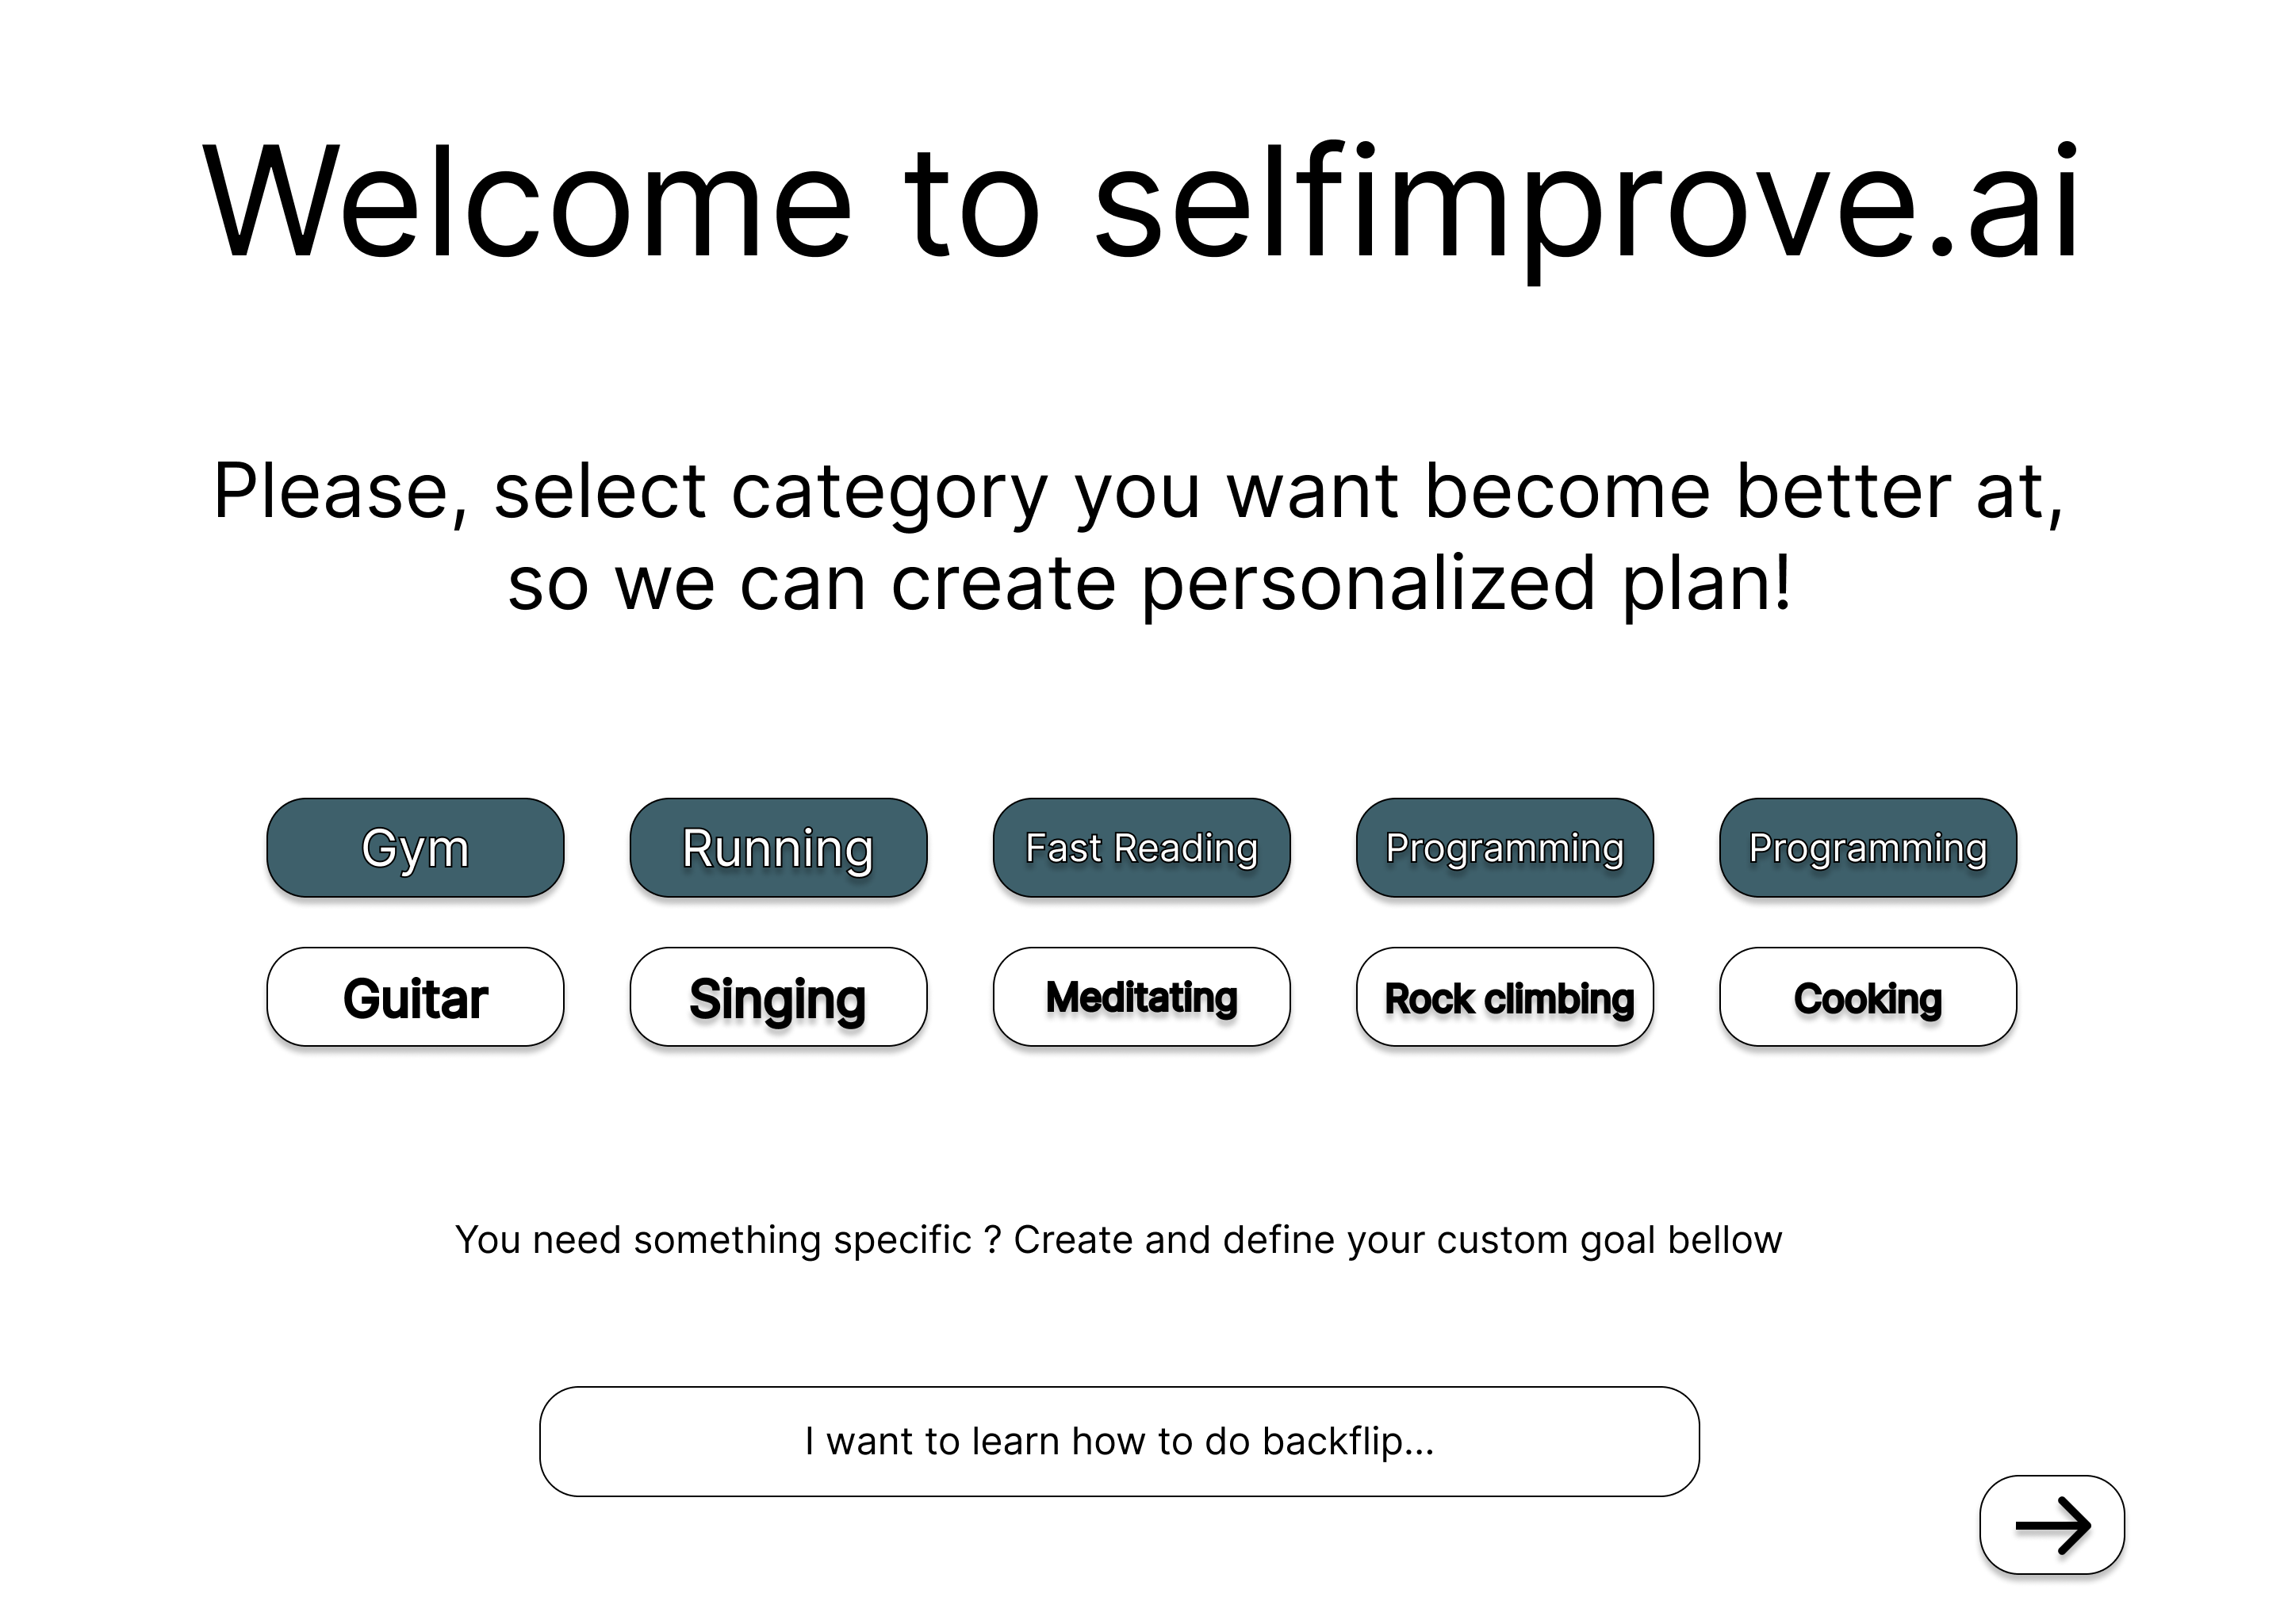
\includegraphics[width=1\textwidth]{Obrazy/prototypy/personalizacja_konta.png}
    \caption{Prototyp ekranu personalizacji konta}
    \label{fig:my_label}
\end{figure}

\begin{figure}[H]
    \centering
    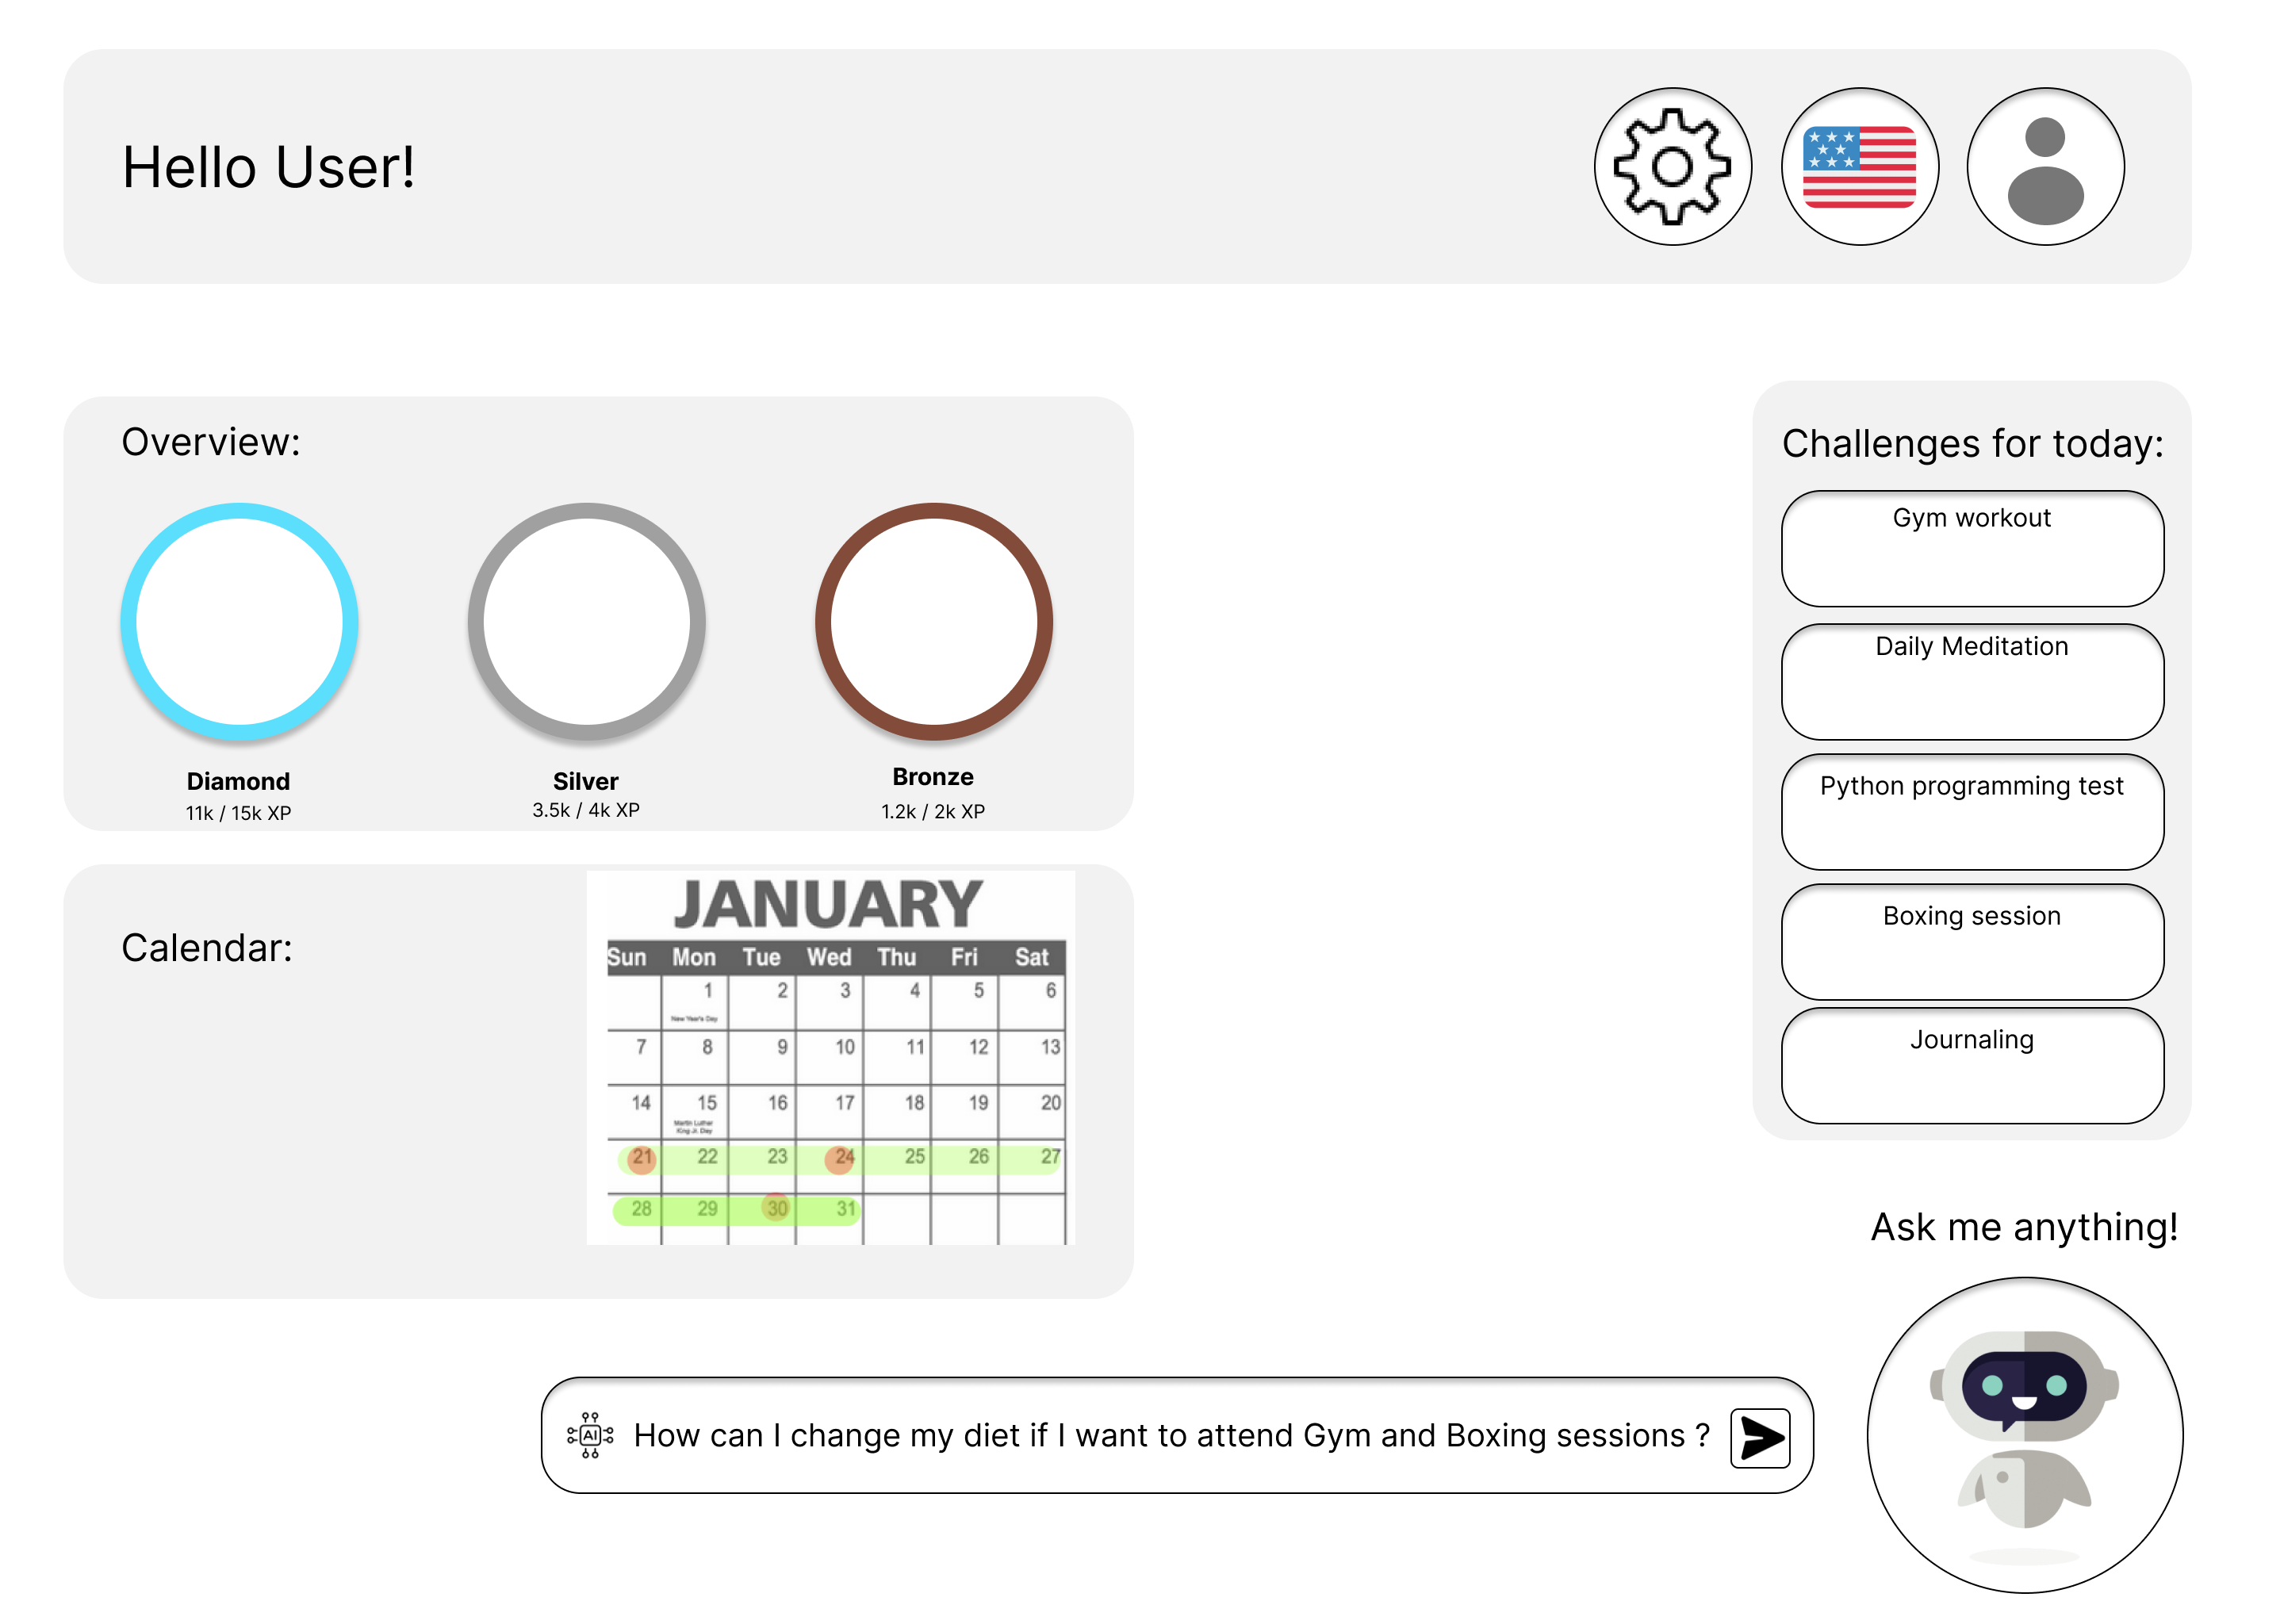
\includegraphics[width=1\textwidth]{Obrazy/prototypy/strona_startowa.png}
    \caption{Prototyp strony startowej}
    \label{fig:my_label}
\end{figure}

\begin{figure}[H]
    \centering
    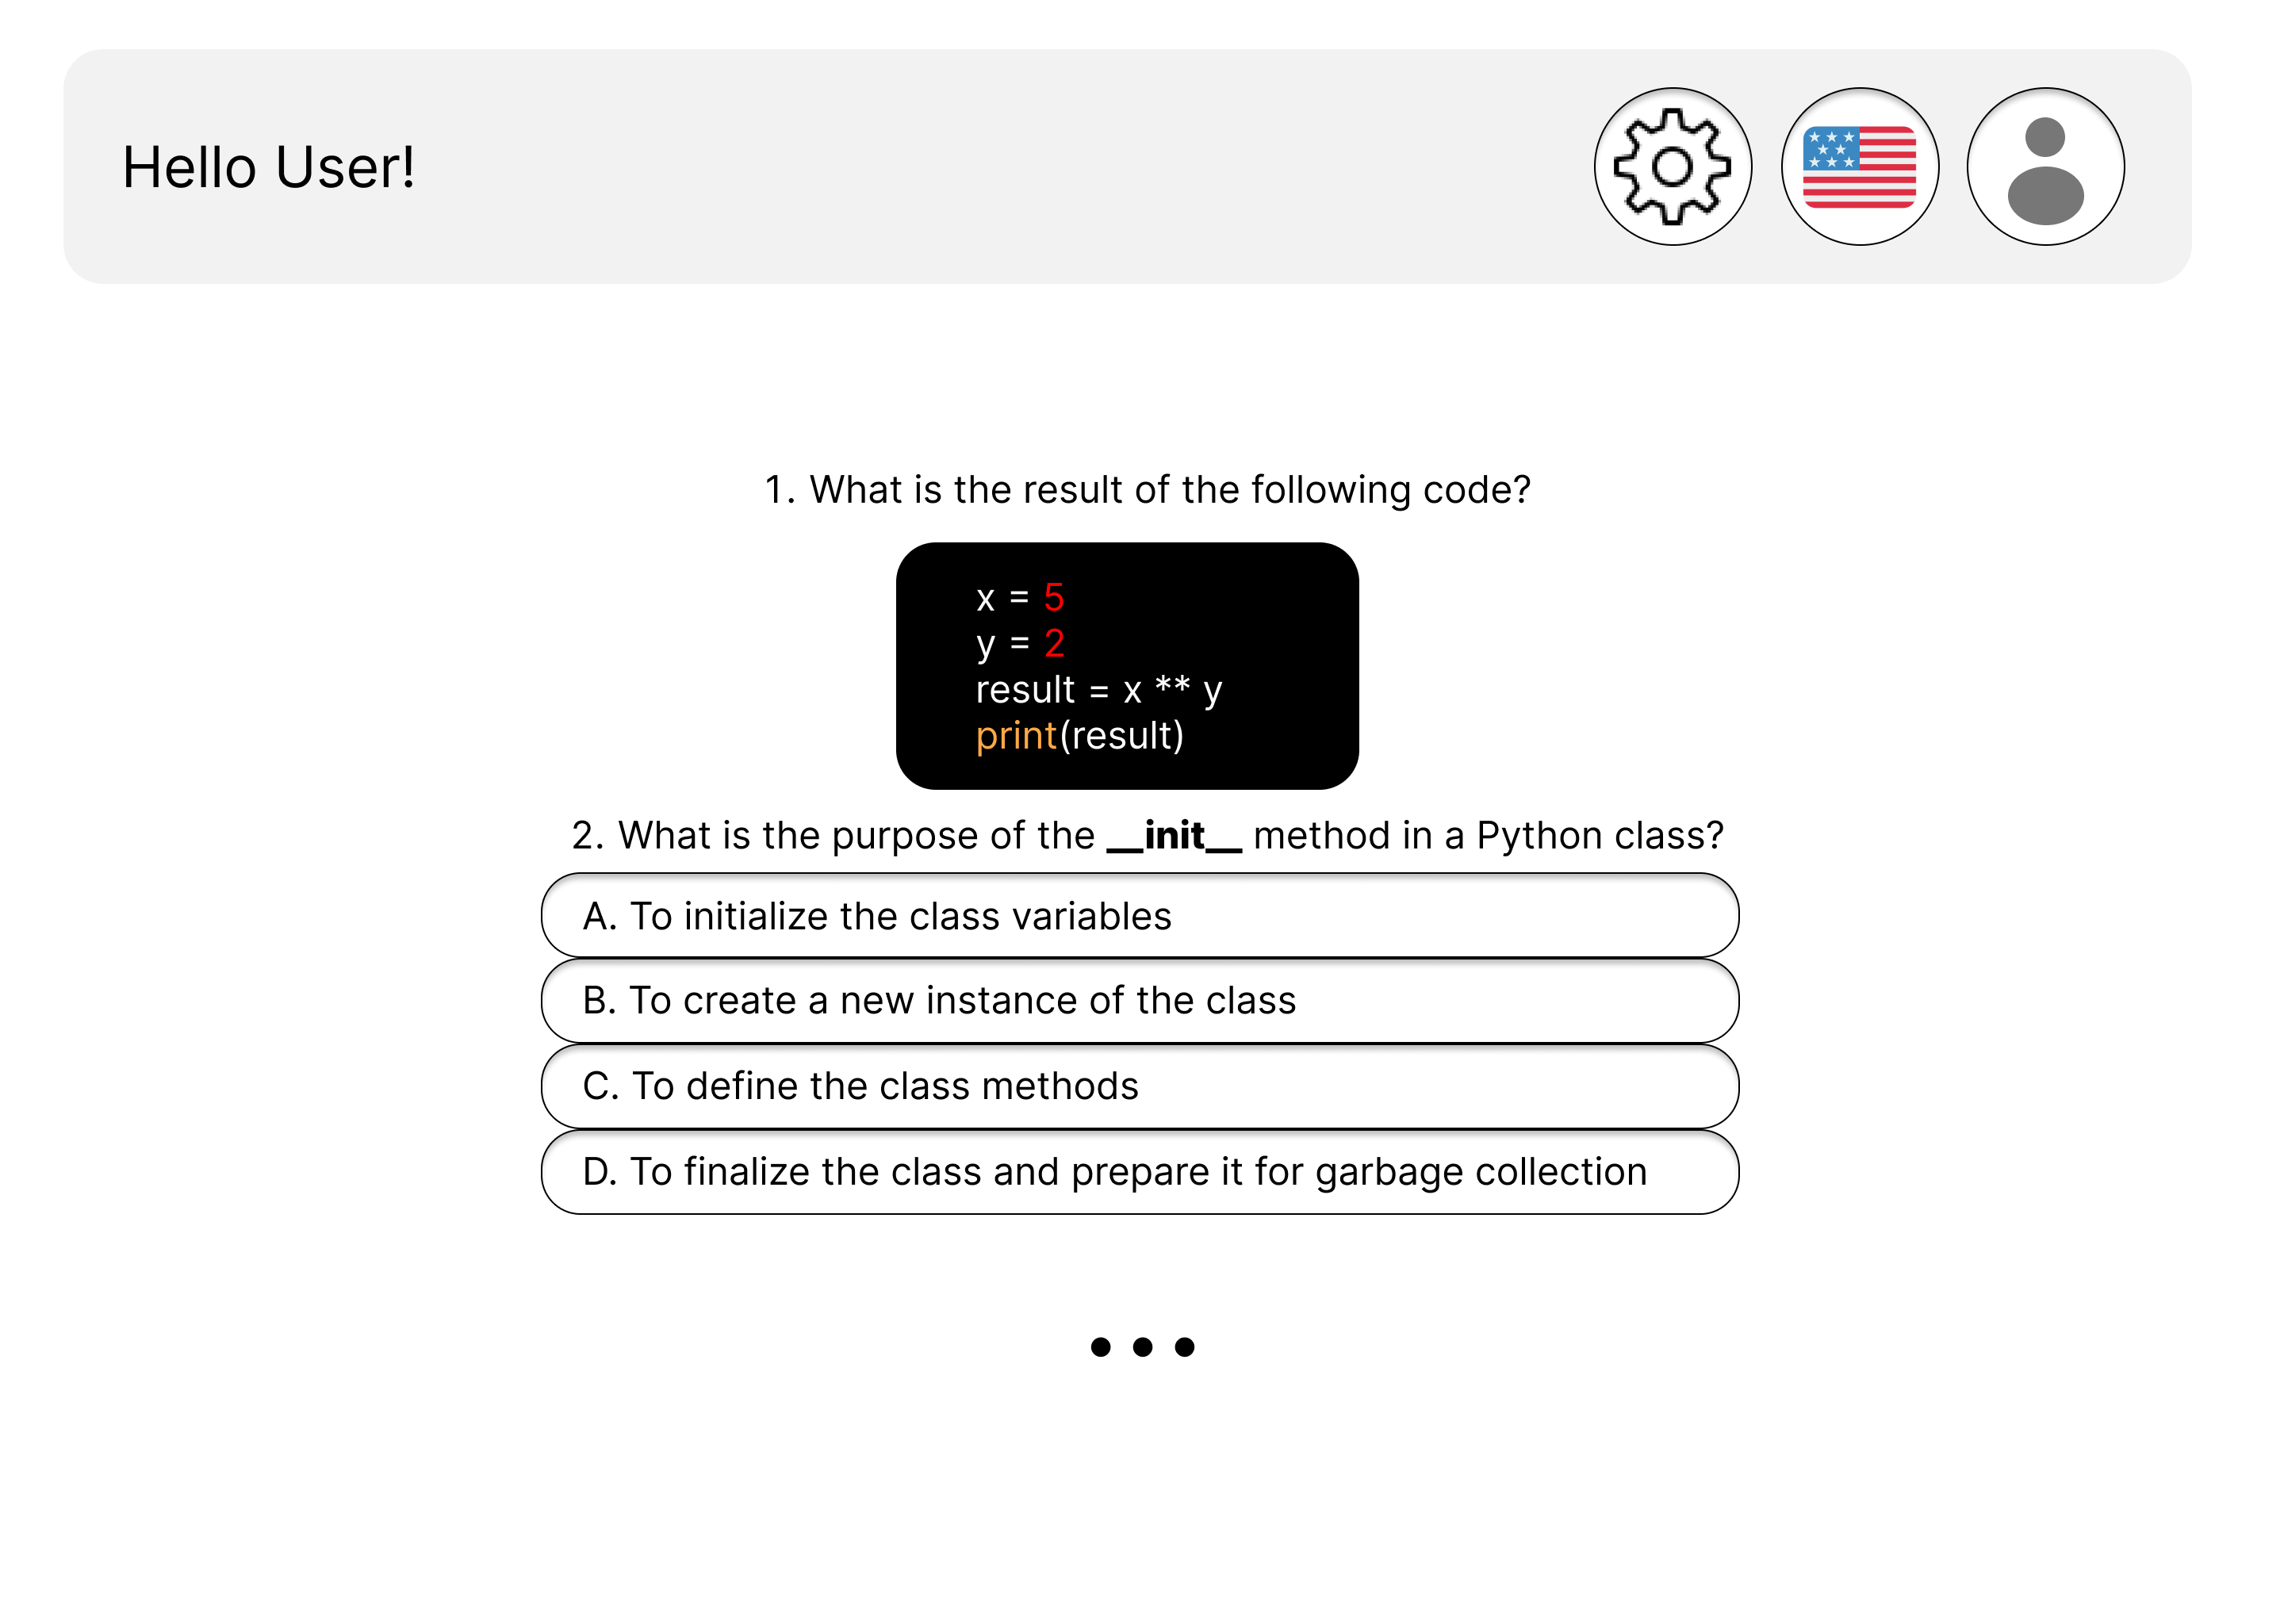
\includegraphics[width=1\textwidth]{Obrazy/prototypy/panel_zadania.png}
    \caption{Prototyp panelu zadania}
    \label{fig:my_label}
\end{figure}

\begin{figure}[H]
    \centering
    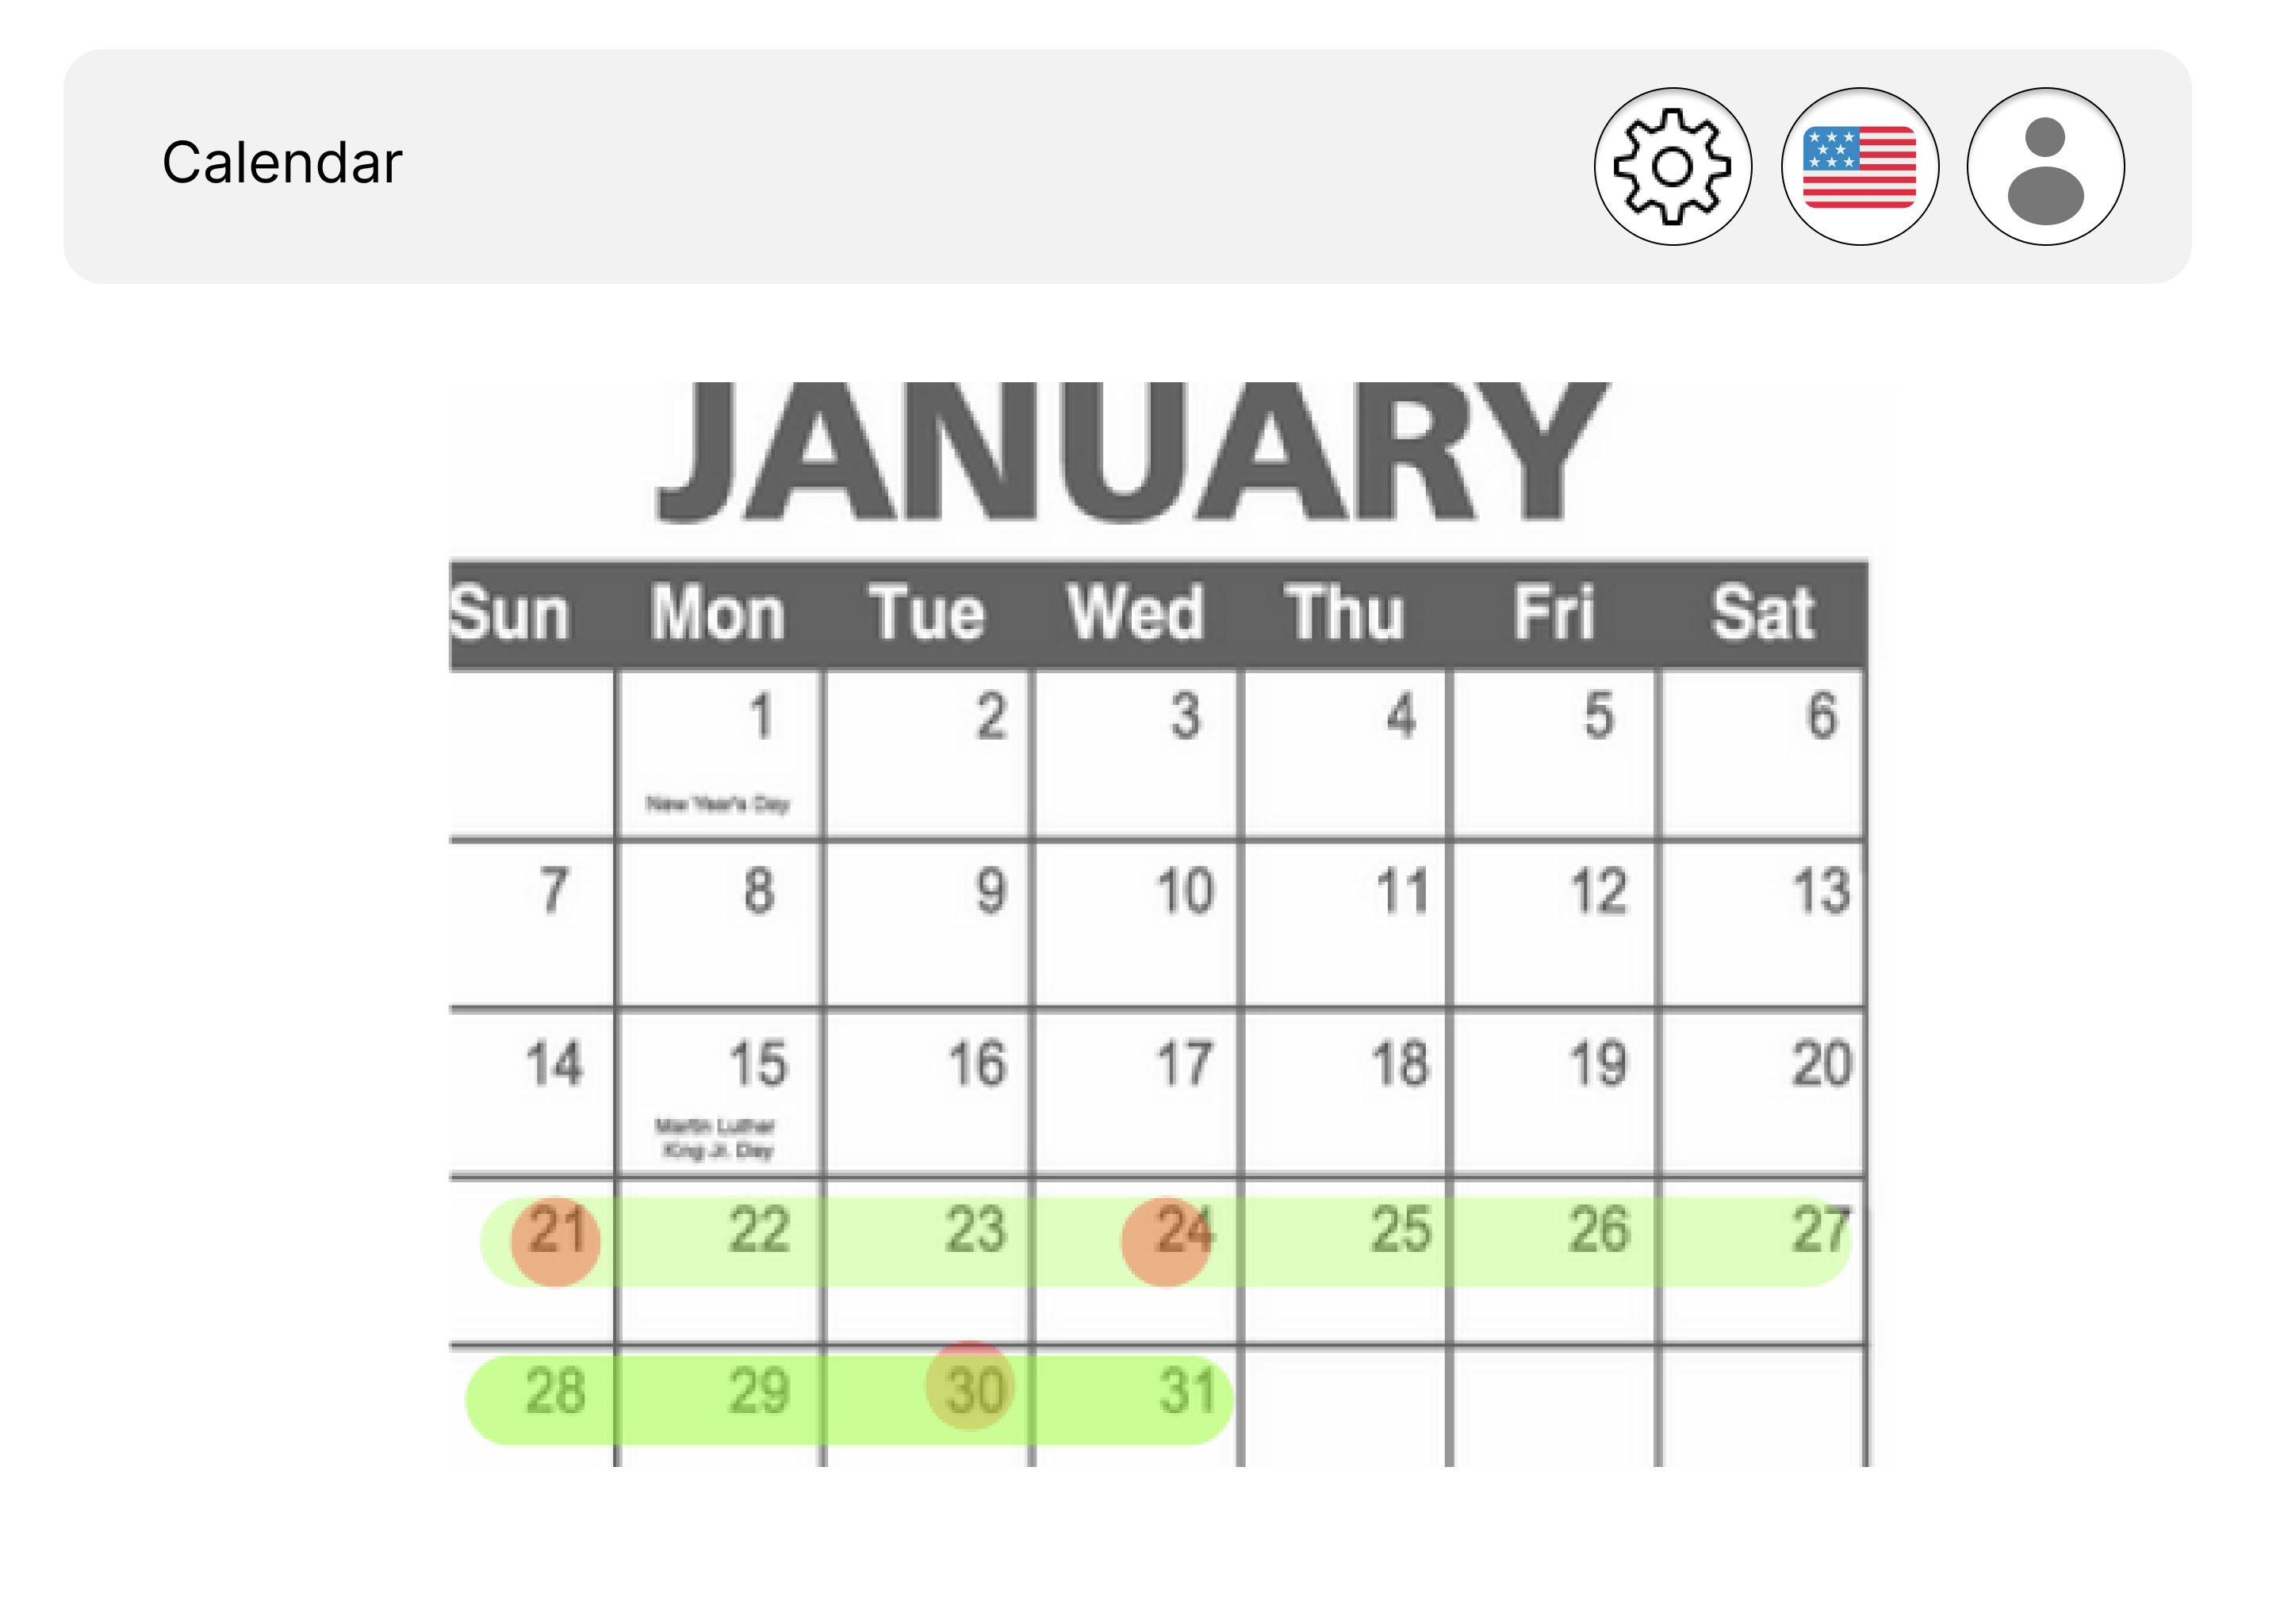
\includegraphics[width=1\textwidth]{Obrazy/prototypy/kalendarz.png}
    \caption{Prototyp kalendarza}
    \label{fig:my_label}
\end{figure}

\begin{figure}[H]
    \centering
    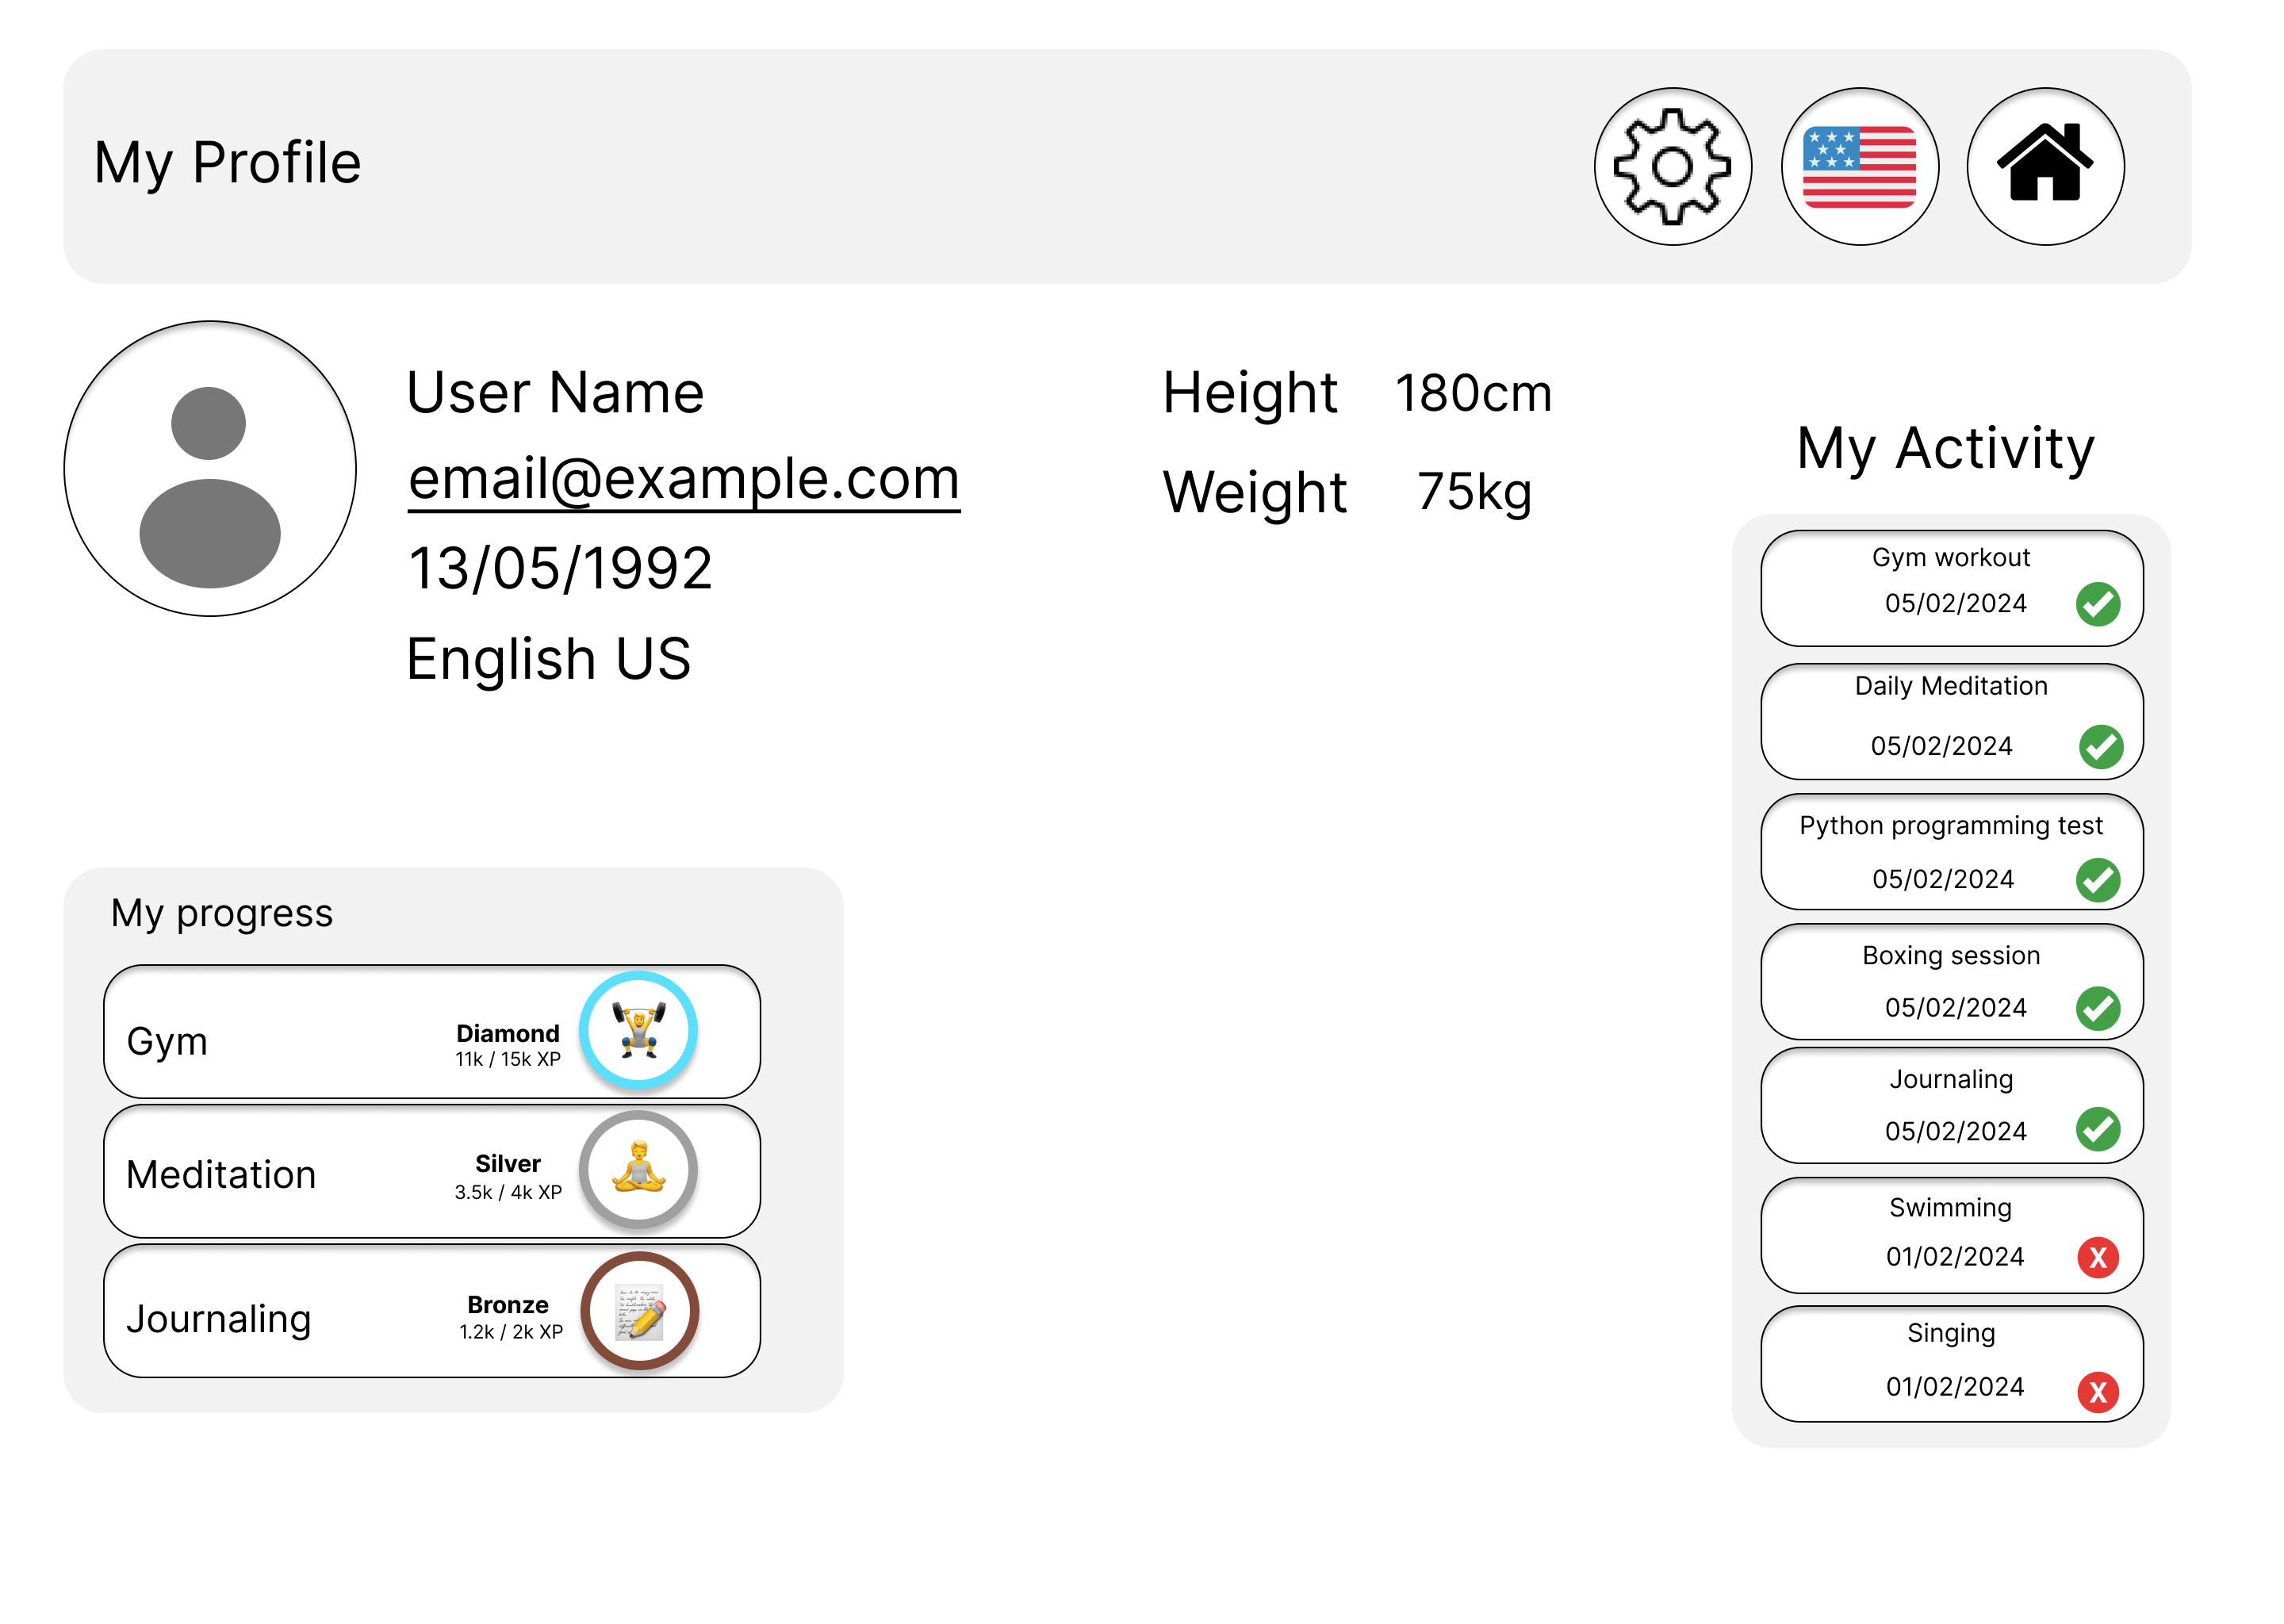
\includegraphics[width=1\textwidth]{Obrazy/prototypy/profil_uzytkownika.png}
    \caption{Prototyp profilu użytkownika}
    \label{fig:my_label}
\end{figure}

\clearpage